\documentclass{buthesis}

\usepackage{hologo}
\usepackage{booktabs}
\usepackage{float} 
\usepackage{amsmath}
\usepackage{svg,graphicx}
\usepackage{tabularx, array, ragged2e}
\newcolumntype{Y}{>{\RaggedRight\arraybackslash}X}
\usepackage[utf8]{inputenc}
\usepackage{newunicodechar}
\usepackage[nottoc]{tocbibind}
\usepackage[titletoc]{appendix}
\setcounter{tocdepth}{2}
\usepackage{listings}
\usepackage{xcolor}
\usepackage{listingsutf8}
\usepackage{import}
\usepackage[ruled,vlined]{algorithm2e}
\usepackage{hyphenat}
\usepackage[final]{microtype}

\usepackage{xurl}
\usepackage{hyperref}

\hyphenpenalty=3000
\exhyphenpenalty=3000
\emergencystretch=2em


\svgsetup{
	inkscapeexe={C:/Program Files/Inkscape/bin/inkscape.exe},
	inkscapelatex=true,
	inkscapearea=page
}


\lstset{
  inputencoding=utf8,
  basicstyle=\ttfamily\small,
  breaklines=true,
  literate=
    {–}{{-}}1 {—}{{---}}1 {…}{{\ldots}}1
    {→}{{$\to$}}1 {←}{{$\leftarrow$}}1 {⇒}{{$\Rightarrow$}}1
    {α}{{$\alpha$}}1 {β}{{$\beta$}}1 {γ}{{$\gamma$}}1 {δ}{{$\delta$}}1
    {π}{{$\pi$}}1 {σ}{{$\sigma$}}1 {τ}{{$\tau$}}1
    {Δ}{{$\Delta$}}1 {Σ}{{$\Sigma$}}1 {Ω}{{$\Omega$}}1
}

\lstset{
  basicstyle=\ttfamily\small,
  breaklines=true,
  breakatwhitespace=true,
  columns=fullflexible,
  keepspaces=true,
  tabsize=2,
  frame=single,
  rulecolor=\color{black!20},
  xleftmargin=0.5em, xrightmargin=0.5em,
  aboveskip=0.75\baselineskip, belowskip=0.75\baselineskip,
  postbreak=\mbox{\textellipsis\space}
}


\newunicodechar{π}{\ensuremath{\pi}}
\newunicodechar{α}{\ensuremath{\alpha}}
\newunicodechar{β}{\ensuremath{\beta}}
\newunicodechar{γ}{\ensuremath{\gamma}}
\newunicodechar{δ}{\ensuremath{\delta}}
\newunicodechar{ε}{\ensuremath{\varepsilon}}
\newunicodechar{θ}{\ensuremath{\theta}}
\newunicodechar{λ}{\ensuremath{\lambda}}
\newunicodechar{μ}{\ensuremath{\mu}}
\newunicodechar{ρ}{\ensuremath{\rho}}
\newunicodechar{σ}{\ensuremath{\sigma}}
\newunicodechar{τ}{\ensuremath{\tau}}
\newunicodechar{φ}{\ensuremath{\varphi}}
\newunicodechar{ω}{\ensuremath{\omega}}
\newunicodechar{Δ}{\ensuremath{\Delta}}
\newunicodechar{Λ}{\ensuremath{\Lambda}}
\newunicodechar{Σ}{\ensuremath{\Sigma}}
\newunicodechar{Ω}{\ensuremath{\Omega}}



\begin{document}

\title{Detecting Interprocedural Software Vulnerabilities Using Causal Deep Learning}
\author{Md Iqbal Hossain Shuvo}

\beforepreface
\prefacesection{Abstract}

Modern software stacks contain long, cross-module execution paths where subtle interactions between functions can create exploitable flaws, yet traditional and most learning based vulnerability detectors continue to operate as opaque classifiers that provide only coarse-grained labels over files or graph representations. This thesis introduces a causal, chain centric approach that couples vulnerability prediction with explicit reconstruction of executable root-to-sink chain across functions and files. The method starts from an augmented code property graph that integrates abstract syntax, control flow, data flow, and interprocedural links, then initializes node features with a pretrained structure aware encoder (GraphCodeBERT) and refines them using a relation-aware graph neural network with Adaptive Causal Contextualization guided by a mined Causal Knowledge Graph prior. A constrained beam search decoder, backed by feasibility checks over control, data, and call or return edges, assembles a single executable chain for each positive decision that respects program semantics, aliasing constraints, and interprocedural dependencies. Experiments on the ReposVul repository-level dataset evaluate detection performance and explanation quality using both standard metrics and specialized criteria. These evaluation criteria encompass the Counterfactual Consistency Score (CCS), the Causal Feature Attribution Measure (CFAM), and additional measures that check whether the chains are valid, cover the relevant interprocedural paths, match reference vulnerability chains, and respond in a sensible way to targeted program edits. This comprehensive evaluation approach ensures robust assessment of model accuracy, interpretability, and causal fidelity. The proposed approach not only achieves strong vulnerability detection performance but also effectively reconstructs a vulnerability chain. This chain explicitly captures the root cause (source), the intermediate propagation steps, and the vulnerable point (sink), and passes comprehensive feasibility checks, exhibiting improved coverage and correct ordering of these critical stages. This explicit root–propagation–sink representation in turn enables high-fidelity interprocedural explanations that align with developers’ diagnostic workflows and support root-cause reasoning in large-scale, heterogeneous software systems.


\prefacesection{Acknowledgments}

I am deeply grateful to my supervisor, Dr. Yasir Malik, for his unwavering support, insightful guidance, and patience throughout the course of this research. His mentorship has been invaluable in shaping both my academic and professional growth. I also wish to express my heartfelt gratitude to my family, whose constant love, encouragement, and understanding have been essential in completing this thesis. 

\figurespagetrue
\tablespagetrue

\afterpreface

\chapter{Introduction}
\label{chap:intro}

Software vulnerability detection remains a critical yet complex challenge in software engineering. Modern digital infrastructure, financial services, scientific workflows, and everyday communication all depend on large, evolving software systems. As these systems scale in size and heterogeneity, contemporary codebases span millions of lines of code and are developed by distributed teams over long periods of time. This growth in complexity increases architectural coupling and the likelihood that subtle defects persist into production. When such defects are exploitable, they become security vulnerabilities that threaten confidentiality, integrity, and availability, and their effects may propagate across dependent components and services~\cite{Li2022Empirical,yang2022natural,Le2024MBU}.

A bug is a defect that causes a program to behave incorrectly or unexpectedly. Not all bugs threaten security. A vulnerability is a defect that an adversary can exploit to violate confidentiality, integrity, or availability. Distinguishing benign errors from exploitable vulnerabilities requires understanding not only the defect itself but also the mechanism by which it can lead to a successful attack. This mechanism can be conceptualized as a chain of causation that begins at a root condition (e.g., untrusted input, unchecked buffer length, use-after-free) and propagates through assignments, parameter passing, return values, aliasing relations, and implicit flows induced by control dependence. The chain becomes exploitable when a tainted or unsafe state reaches a sensitive sink, such as a buffer write, command/SQL execution, deserialization routine, or privileged operation. Executability depends on dominance and post-dominance of guards, exceptional paths, resource lifetimes, and other feasibility constraints. This thesis therefore treats vulnerabilities as root→propagation→sink mechanisms to be reconstructed and validated end to end.

Traditional vulnerability detection techniques provide important, but incomplete, coverage of this problem space. \emph{Static analysis} examines code without executing it, relying on rule-based systems, type reasoning, data-flow frameworks, and abstract interpretation to infer program behaviour at scale~\cite{Allix2024,Ruiz2023,taviss2024asm2seq}. \emph{Dynamic analysis} executes programs with concrete or instrumented inputs to observe runtime behaviour directly, often using monitoring, tracing, or sandboxing to detect anomalous states~\cite{yagemann2021arcus,cheng2022path}. In practice, these approaches are complemented by \emph{fuzzing} and penetration testing, which attempt to exercise programs under diverse or adversarial inputs in order to trigger faults and expose exploitable conditions. Static analysis offers broad coverage but tends to over-approximate feasible execution paths, producing false positives and limited insight into concrete exploitability, while dynamic analysis, fuzzing, and penetration testing provide high-fidelity traces but often struggle with input coverage, scalability, and reproducibility on large, modular systems~\cite{Li2022Empirical,Le2024MBU}. Recent years have seen a substantial shift toward \emph{data-driven approaches} for software vulnerability detection. These methods, which include machine learning and deep learning based models, aim to automate vulnerability discovery by learning patterns from code representations such as token sequences, abstract syntax trees, control-flow graphs, and data-flow graphs. These heterogeneous representations are unified within Code Property Graphs (CPGs) that integrate syntactic, semantic, and control/data flow information via typed nodes and edges. Graph Neural Networks (GNNs) utilize relation-aware message passing and type-specific attention mechanisms to propagate information over these graphs, enabling fine-grained vulnerability classification and localization \cite{Zhou2019,hin2022linevd,Chakraborty2020}. Pretrained models such as GraphCodeBERT enrich token embeddings with data-flow aware context and thereby improve generalization, while frozen language-model representations, when combined with relation-aware GNNs, enable effective propagation of causally relevant evidence over heterogeneous code graphs, strengthening learning-based vulnerability detection.

Despite this progress, existing static, dynamic, fuzzing, and data-driven techniques remain largely \emph{correlation-centric} and are not sufficient to capture the full causal structure of real-world vulnerabilities. Traditional deep learning models tend to rely heavily on statistical associations in training data, often capturing superficial patterns rather than the underlying causes of vulnerabilities. They typically focus on isolated statements or small subgraphs that are predictive of the vulnerability label and emphasize \emph{where} a flaw is likely to occur, rather than \emph{how} it emerges and propagates through interacting control and data flows~\cite{Li2022Empirical,yang2022natural}. This correlation-centric bias produces several limitations: models can become sensitive to dateset-specific artifacts such as naming conventions or formatting and may fail under benign transformations such as refactoring, formatting changes, or identifier renaming~\cite{Li2022Empirical,yang2022natural}. Modeling such behaviors requires reasoning not only about local syntax and intra-procedural structure but also about interprocedural semantics, including call and return edges, argument-to-parameter bindings, return-to-caller relationships, and conservative aliasing across function and module boundaries~\cite{Le2024MBU}. Existing vulnerability detection techniques, including static and dynamic analysis, fuzzing and penetration testing, and modern data-driven detectors, therefore provide important but incomplete coverage of this interprocedural behaviour. Classical static, dynamic, and fuzzing-based solutions are effective at finding local defects or triggering specific failure scenarios, but they rarely find interprocedural vulnerability. Similarly, most data-driven detectors are trained to classify localized code regions or limited graph neighborhoods and tend to focus on point wise predictions of \emph{where} a vulnerability may occur, rather than modeling \emph{how} vulnerable state propagates across functions and modules in a causally meaningful way~\cite{Li2022Empirical,yang2022natural,Le2024MBU}.

In real software systems, vulnerabilities often arise from complex interactions that span multiple functions, modules, or files. Tainted input may flow through several layers of wrapper functions before reaching a sensitive sink; resource management errors may involve initialization in one component and misuse in another; and access-control checks may be applied inconsistently across different call paths. These behaviours are further complicated by the use of shared libraries, callbacks, framework conventions, and configuration-driven control flow, where the relevant control and data dependencies are distributed across APIs, modules, and sometimes even language boundaries. As a result, the conditions that make a defect exploitable often depend on long, cross-cutting chains of calls and data transformations that are only partially visible in any single local context. Existing static, dynamic, fuzzing, and data-driven techniques typically approximate these patterns using limited context or heuristics~\cite{Li2022Empirical,Le2024MBU}.

To address these challenges, this thesis adopts a \emph{causal and context-aware} perspective on vulnerability detection. In this approach, \emph{context awareness} refers to the capability of a model to understand how program elements relate not only syntactically, but also semantically, through control flow, data dependencies, and functional interactions~\cite{yamaguchi2014cpg,guo2021graphcodebert}. Vulnerabilities often do not originate from a single isolated statement; instead, they emerge from the interplay of multiple operations over time and across function boundaries, so capturing this semantic context is essential for reconstructing meaningful explanations of vulnerability behaviour, especially in interprocedural scenarios~\cite{Le2024MBU}. At the same time, the thesis builds on principles from \emph{causal inference}, which seek to distinguish true cause–effect relationships from spurious correlations and have motivated recent causal and explainable approaches to vulnerability detection~\cite{Cao2024Snopy,Kuang2024KSEM,Rahman2024ICSE,Chu2024ISSTA}. In the context of vulnerability detection, the integration of causal reasoning within program analysis is both strategically advantageous and fundamentally essential. Effective remediation hinges on accurately identifying the specific code elements and propagation pathways that are causally responsible for vulnerabilities. Accordingly, this thesis adopts an approach that develops a context-aware, data-driven causal framework to reconstruct interprocedural root-to-sink vulnerability propagation paths within source code. This approach seeks to harmonize vulnerability prediction with executable, causally grounded explanations, elucidating not only the presence of vulnerabilities but also the precise manner in which they emerge and disseminate across functions and modules. Such causally informed interpretations provide a necessary foundation for trustworthy, actionable vulnerability diagnostics and remediation guidance.

\section{Research Gaps}
\label{sec:intro-gaps}

Software vulnerability detection has advanced considerably, yet several critical gaps remain in current data-driven and interprocedural analysis techniques.

\medskip
\noindent\textbf{Gap 1: Causal deficiency and generalization:}  
Many data-driven detectors learn superficial statistical correlations rather than the underlying flaw mechanisms. Their predictions often deteriorate under benign code refactorings and cross-project generalization, reflecting insufficient causal grounding and poor robustness to distribution shifts~\cite{Li2022Empirical,yang2022natural}. 

\medskip
\noindent\textbf{Gap 2: Interprocedural reasoning and chain reconstruction:}  
Most existing approaches focus on individual functions or limited intra-procedural slices and lack interprocedural dependencies~\cite{Le2024MBU}, thereby failing to reconstruct executable root-to-sink vulnerability propagation chains across large, modular software systems.

\section{Research Objectives}
\label{sec:intro-objectives}

To systematically advance the understanding and detection of software vulnerabilities, this thesis focuses on following research questions and corresponding objectives. 
\subsection*{Research Questions}
\noindent\textbf{RQ 1:}  
How can a program representation be designed that faithfully captures interprocedural control and data dependencies in a form that supports executable, root-to-sink causal analysis across functions, files, and modules?

\noindent\textbf{RQ 2:}
How can a context-aware causal reasoning approach systematically construct executable interprocedural vulnerability chains that are viable, minimal, and consistent with the underlying control flow, data dependencies, and aliasing relationships?

\subsection*{Research Objectives}

To achieve the goal of reconstructing executable interprocedural vulnerability propagation chains, this thesis pursues the following research objectives.

\medskip
\noindent\textbf{O 1:}  
Design a program representation that captures interprocedural control and data dependencies, combining structures such as Abstract Syntax Trees (ASTs), Control-Flow Graphs (CFGs), Data-Flow Graphs (DFGs), and Program/Code Property Graphs (PDG/CPG), in a form suitable for root-to-sink causal analysis across functions, files, and modules.

\medskip
\noindent\textbf{O 2:}  
Create a constraint-based approach to generate executable, interprocedural vulnerability chains, explicitly representing control flow, data dependencies, and aliasing to produce chains that are viable, minimal, and mechanically valid.

\medskip

This thesis reconstructs executable interprocedural root-to-sink vulnerability propagation chains from real-world vulnerable repositories. The codebase is parsed into Abstract Syntax Trees, Control-Flow Graphs, and Data-Flow Graphs, which are integrated into a unified Program/Code Property Graph augmented with interprocedural semantics (call/return edges, argument$\rightarrow$parameter mappings, return$\rightarrow$caller links, and conservative aliasing) so that candidate root-to-sink paths can be followed across functions, files, and modules. Nodes in this heterogeneous graph are encoded using a structure-aware pretrained model (GraphCodeBERT) combined with structural features, and these embeddings are refined by a graph-based encoder equipped with attention, Adaptive Causal Contextualization (ACC), and a Causal Knowledge Graph (CKG)~\cite{Zheng2023CausalKG} prior. On top of this encoder, a constrained beam search decoder explores feasible control- and data-flow paths to assemble executable root-to-sink chains consistent with the interprocedural semantics.

\section{Contributions and Significance}
\label{sec:intro-contrib}

This research transforms vulnerability explanation from localized, retrospective feature highlights into a unified, executable interprocedural causal chain that traces the propagation from root cause to exploitable sink. This approach helps bridge the gap between traditional static and dynamic analyses, fuzzing and penetration testing, and modern data-driven vulnerability detectors, aligning automated analysis more closely with the complexity of large, modular software systems. The research makes model predictions interpretable by reconstructing how untrusted input enters the system, travels through control and data dependencies across functions, avoids or skips sanitization, and reaches a vulnerable operation. These chains give developers clear, traceable proof of a vulnerability's existence, as well as clear instructions on where to find it and what to do to fix it. This transforms black-box detections into actionable and verifiable information. This enhances the reliability, transparency, and practical utility of learning-based vulnerability detection, contributing to software security in real-world environments.

Taken together, this problem framing and methodological perspective give rise to the following contributions in interprocedural, causality-aware software vulnerability analysis.

\medskip
\noindent\textbf{C1 - A chain-centric interprocedural program representation:}  
This thesis extends the code property graph by integrating explicit interprocedural semantics, preserving control and data dependencies across functions and files to enable reconstruction of executable root-to-propagation-to-sink chains.

\medskip
\noindent\textbf{C2 - Interprocedural causal vulnerability chain construction:}  
A context driven causal pipeline that constructs explicit interprocedural root-to-sink vulnerability chains. This approach constructs the full propagation path (root→propagation→sink) as the main explanatory unit.



\section{Thesis Outline}
\label{sec:intro-outline}

This thesis is structured as follows. Chapter 1 introduces the problem context, articulates the research gaps, formulates the research questions and objectives, and summarizes the main contributions. Chapter 2 reviews related work in the software vulnerability detection domain. Chapter 3 describes the methodology, including dataset preparation, interprocedural graph construction, chain-centric representation, and the model architecture with its decoding pipeline. Chapter 4 presents the experimental setup, and detailed results focusing on detection accuracy, chain quality, causal analyses, robustness, and case studies. Chapter 5 concludes with key findings, implications, limitations, and future research directions. Appendices provide supplementary materials such as algorithms, model equations, metrics, extended results, and reproducibility details.



\chapter{Literature Review}

The growing need for more reliable and interpretable software vulnerability detection methods has driven extensive exploration of deep learning (DL) based approaches in recent research. These methods aim to automate the identification of vulnerabilities by learning patterns from code representations, often outperforming traditional static and dynamic analysis. However, despite their success, deep learning models still face challenges in scalability, generalizability, and transparency. To address these issues, researchers have investigated both the refinement of DL-based detection techniques and the development of methods to enhance model explainability and causal reasoning capability. This pursuit of more robust and interpretable models leads directly to the exploration of advanced DL architectures and explainability techniques discussed in this chapter.

\section{Related Works}

\subsection{Static and Dynamic Analysis Techniques}

Static analysis examines software artifacts without executing them and seeks to reason soundly or semi-soundly about all possible program behaviours. Classical approaches rely on lattice-based data-flow frameworks, abstract interpretation, and type- or effect-based reasoning to approximate control and data dependencies at scale \cite{yamaguchi2014cpg,Chakraborty2020}. Their precision depends on sensitivities to control flow, calling context, execution paths, and heap or field abstractions. Interprocedural static analysis, in particular, requires accurate call-graph construction, supported by techniques such as Class Hierarchy Analysis, Rapid Type Analysis, and points-to analysis to resolve aliasing and dynamic dispatch \cite{Xia2023,Liu2020}. These analyses operate over canonical program representations: Abstract Syntax Trees (ASTs) encode syntactic structure, Control-Flow Graphs (CFGs) capture feasible execution order and branching, Data-Flow Graphs (DFGs) trace definition–use chains of variable values, and Program Dependence Graphs (PDGs) unify data and control dependencies to support slicing and taint tracking. The Code Property Graph (CPG) integrates AST, CFG, and DFG into a heterogeneous multigraph and has been widely adopted to support scalable, interprocedural vulnerability queries from sources to sinks \cite{yamaguchi2014cpg}.

Despite their ability to detect potential issues early, classical static analyses routinely suffer from false positives due to conservative over-approximation of sanitization logic, aliasing, reflection, and dynamic dispatch \cite{Ruiz2023,Allix2024}. Comparative studies of widely used static analyzers, such as Flawfinder, RATS, Cppcheck, SpotBugs, and PMD, report substantial variability in detection rates and false-positive profiles across languages and vulnerability categories \cite{Kaur2020comparative}. These limitations have motivated integration of machine learning and deep learning into static analysis pipelines. For example, IRIS combines large language models (LLMs) with static analysis to infer taint specifications and expand coverage of vulnerability patterns while reducing false discoveries, outperforming rule-centric tools such as CodeQL on several benchmarks \cite{Li2024IRIS}. Other hybrid approaches use ML classifiers to post-process static warnings, filter likely false positives, or prioritise alerts for manual inspection, thereby improving scalability and analyst productivity \cite{hu2023hybrid}. Static analysis thus remains a foundational component that provides structured, semantically rich program views to downstream learning-based detectors, even as its limitations on complex, rapidly evolving, and domain-specific codebases remain an open challenge \cite{Xia2023,Chakraborty2020}.

Dynamic analysis complements static reasoning by monitoring concrete or symbolic program executions to detect vulnerabilities at runtime. Representative techniques include fuzzing, which automatically mutates inputs to explore diverse execution paths; runtime sanitizers, which instrument code to detect memory safety violations and undefined behaviour; and symbolic or concolic execution, which uses constraint solvers to systematically explore feasible paths leading to potential faults \cite{yagemann2021arcus,yagemann2021automated}. Dynamic methods produce high-fidelity witness traces that are directly actionable for debugging and exploit validation, but they are constrained by path explosion, environment modelling issues, and limited input or configuration coverage, especially in large-scale interprocedural systems \cite{yagemann2021arcus}. To mitigate these limitations, recent work has proposed hybrid static–dynamic workflows in which machine learning and reinforcement learning guide fuzzing campaigns, prioritise target functions, or learn path selection heuristics from execution feedback, thereby improving coverage and discovery rates \cite{xu2023mlforfuzzing,tufano2022adaptive}. Overall, static analysis offers scalability and whole-program coverage, whereas dynamic analysis provides precise execution evidence; their integration, increasingly mediated by data-driven techniques, forms a central strand in contemporary research on automated software vulnerability detection.


\subsection{Deep Learning Based Techniques}

Deep learning is reshaping many areas of computer science, and graph neural networks (GNNs) have rapidly shown strong performance in software vulnerability detection \cite{Chakraborty2020,Liu2020,Yaqin2020,hin2022linevd}. By modeling code as graphs whose nodes represent program elements and edges encode syntactic and semantic relations, GNN-based models can capture complex software dependencies and localize vulnerable statements, for example in the line-level setting demonstrated by Hin et al.~\cite{hin2022linevd}. However, many of these models operate as opaque “black boxes,” making it difficult to understand why a particular code fragment is classified as vulnerable \cite{li2023vulanalyzer,mosolygo2021towards}, even when prediction accuracy is high. In security-critical contexts, this lack of transparency is problematic: developers must understand \emph{why} a vulnerability is reported in order to implement appropriate fixes, and recent policy initiatives, such as the U.S.\ Executive Order on safe, secure, and trustworthy AI, explicitly emphasize the need for reliable and explainable AI behaviour in high-stakes systems \cite{USGov2023}.

Zhou et al. \cite{Zhou2019} conducted a systematic empirical study of design factors that influence the performance of deep learning based vulnerability detectors. They constructed two datasets capturing both data and control dependencies for 126 vulnerability types and implemented a Joern based detection pipeline to enable controlled comparisons. Their experiments quantified the impact of several key choices, including techniques for handling class imbalance, the inclusion of control dependence information in code representations, and the selection of neural network architectures, on downstream detection accuracy. The results provide practical guidance for building effective DL based vulnerability detection systems, but the work remains correlation oriented and does not explicitly incorporate causal deep learning or formal causal reasoning principles.


Li et al. \cite{Li2022Empirical} performed empirical research on deep learning (DL) models for vulnerability detection. On Devign and MSR data, they polled and replicated nine state-of-the-art (SOTA) models. They looked at and examined model capabilities (agreement, variability, performance on several vulnerability categories, and difficulties in addressing particular code aspects). They investigated how model performance responded to project mix and training data size. They identified significant code aspects applied for prediction using model explanation tools. The main contribution of the authors was a thorough investigation of models of deep learning vulnerability detection. For assessing and contrasting several deep learning models for vulnerability identification, this research offers a useful standard. Still, this study paid little attention to causative factors. The authors urged more investigation on code patterns, possible inclusion of causal detection for better generalization, and addressing of the shortcomings of present model interpretation techniques.

\subsection{Causal Reasoning and Causal Deep Learning Techniques}

Conventional deep learning based vulnerability detectors are highly sensitive to spurious correlations and dataset shift. VulCausal, presented by Kuang et al.~\cite{Kuang2024KSEM}, introduces a causal perspective by defining a structural causal model over user-defined identifiers, API library calls, and code structure, then applying backdoor-style adjustments during reasoning to suppress confounding and remove misleading associations. This yields more stable and accurate vulnerability predictions than correlation-driven baselines, but the approach still faces practical limitations, including scalability to very large codebases, limited language coverage, and the absence of explicit executable causal chains beyond improved metrics. More broadly, such methods highlight both the promise of causal inference for vulnerability detection and the substantial modelling effort required, in line with ongoing work on learning more robust, causally grounded optimizers and representations~\cite{Zelikman2023}.

Le et al. \cite{Le2024MBU} examined how existing deep learning based detectors handle vulnerabilities that span multiple basic units of code (MBUs) and showed that models trained and evaluated at the individual basic unit (IBU) level systematically struggle with such cases, overstating accuracy by focusing on isolated units. Although the work does not employ explicit causal reasoning, it provides a detailed characterization and taxonomy of MBU vulnerabilities and analyses their incidence and detection accuracy in modern DL based detectors. The main contribution is a framework for correctly integrating MBU vulnerabilities into DL based detection pipelines, underscoring the need to evaluate models across a spectrum of granularities, which is particularly important in contemporary multi file, multi module software systems. Complementary efforts, such as Nong et al.\ \cite{Nong2023ICSE} on authentic vulnerability generation via pattern mining and deep learning, and Woo et al.\ \cite{Woo2023USENIX} on identifying 1 day vulnerabilities in reused open source components, further refine understanding of vulnerability types and their prevalence in real world code.

Cao et al. \cite{Cao2024Snopy} introduced Snopy, a deep learning method combining change-based sample denoising using vulnerability fixing commits with causal graph learning to enhance vulnerability detection. Snopy employs a Causality Aware Graph Attention Network and Feature Caching Scheme to focus on causal features while suppressing spurious ones. This approach provides a principled way to distinguish causal from non-causal code elements, improving robustness beyond correlation-based detectors. While challenges remain in generalization and spurious correlation mitigation, Snopy represents an important advance toward causal vulnerability detection.

Ganz et al. \cite{Ganz2024} addressed key practical challenges in ML-driven vulnerability detection by focusing on data quality, model interpretability, robustness, and context sensitivity. They introduced novel neural code augmentation to enhance datasets and leveraged dynamic program analysis to evaluate explanation methods. Their causal learning-based bias assessment framework helped reduce confounding effects and improve detection robustness. This work advances learning-based vulnerability detection toward practical relevance by emphasizing data quality and interpretability. Related work by Suneja et al. \cite{suneja2021probing} and Yu et al. \cite{yu2023counterfactual} further explores model interpretability through prediction-preserving input minimization and counterfactual analysis, respectively.

Rahman et al. \cite{Rahman2024ICSE} introduced CausalVul to address the lack of robustness and out-of-distribution generalisation in deep learning based vulnerability detection. They modelled the relationships between code features and vulnerability labels with a causal graph, then used do-calculus and the backdoor criterion in a two-stage pipeline to identify and suppress spurious correlations while preserving causally relevant features. This causal adjustment yields models that rely less on dataset-specific artefacts and more on mechanisms genuinely associated with vulnerabilities, improving both resilience and generalisation. The work represents a clear step toward causal deep learning for vulnerability detection by explicitly targeting false correlations through principled causal inference tools.
 
Chu et al. \cite{Chu2024ISSTA} addressed the lack of explainability in Graph Neural Networks (GNNs) for vulnerability identification. Using counterfactual reasoning, a type of causal inference, CFExplainer aimed to identify minimal changes to the input code graph that would influence the GNN prediction. This improved explainability by focusing on behaviours that alter the outcome and so provides a "what-if" analytical capability. The approach finds a minimum disruption in the code graph by inverting the prediction of the GNN. This provides developers with actionable insights and guides the necessary modifications to remediate the vulnerability. The primary contribution of the authors was the development of a counterfactual explanation method for GNN-based vulnerability discovery. Counterfactual thinking helps developers find a more reasonable and workable argument. A better basis for understanding the application of counterfactual reasoning in explainable artificial intelligence is provided by the work of Lucic et al. \cite{lucic2022cf}.

Islam et al. \cite{Islam2024} proposed T5-GCN for vulnerability categorization, localization, and root cause identification by combining graph convolutional networks with a T5-based large language model. Although the work uses the term “root cause,” it does not employ causal deep learning, causal inference, or formal causal reasoning; instead, it relies on DeepLift-SHAP attribution scores to identify tokens that most strongly contribute to the model’s prediction, providing an attribution-based explanation of the vulnerability. The main contribution lies in coupling GCNs with an LLM for code and using explainability techniques to highlight likely root-causing code fragments alongside vulnerability type, location, and a brief static description. This line of work aligns with growing interest in LLM-based code analysis and optimisation \cite{Zelikman2023} and complements efforts such as Pearce et al.\ \cite{pearce2025asleep}, who assess the security of code produced by GitHub Copilot, indicating the broader potential of LLMs in vulnerability detection and secure software engineering.

Cao et al. \cite{Cao2024Coca} presented Coca, a framework to enhance the causality and robustness of Graph Neural Networks (GNNs)-based vulnerability detection systems. Coca used dual-view causal inference, that is, factual and counterfactual reasoning, to pinpoint code statements most likely to be decisive for vulnerability discovery. This method showed a sophisticated use of causal ideas to solve constraints in robustness and explainability observed in past GNN-based detectors. It also underlined the difficulties in juggling concision with effectiveness in explanations. Coca trains GNNs less prone to false correlations and more focused on real vulnerability traits by means of combinatorial contrastive learning. The Explainer component generates succinct and powerful explanations using dual-view causal inference. Using supervised constrastive learning, the system is taught to identify the bug in all versions and distinguish between buggy and non-buggy code. It discovers a flaw and then employs factual and counterfactual thinking. This is a framework enhancing the causality and dependability of GNN-based vulnerability detection systems. 

\subsection{Explainability and Interpretability Techniques}

Nguyen et al. \cite{nguyen2024} introduced GAVulExplainer, one of the earliest efforts to enhance explainability in deep learning-based vulnerability detection. This model-agnostic framework applies to various GNN detectors and uses genetic algorithms to identify subgraphs that most influence a model’s prediction by isolating coherent subsets of the Code Property Graph responsible for labeling vulnerabilities. Explanation quality is evaluated with a fidelity metric, and users can adjust explanation size to balance conciseness and completeness. While GAVulExplainer significantly advances interpretable GNN vulnerability detection, it focuses on influential subgraphs rather than explicitly modeling causal relationships between code features and vulnerabilities. Nonetheless, it emphasizes the critical role of explanation fidelity for effective remediation and fostering developer trust.

Li et al. \cite{li2023vulanalyzer} presented Vulanalyzer, a deep learning based framework that targets explainable binary vulnerability detection, a challenging setting due to low level representations and sparse semantic cues. The model combines sequential and topological learning to approximate program execution in assembly, using recurrent units and graph convolutions to preserve instruction semantics and control flow, in line with recent work on functional summaries of assembly code \cite{taviss2024asm2seq}. A multi head attention mechanism highlights influential instructions and basic blocks, guiding developers toward code regions the model considers most indicative of a vulnerability and thereby improving interpretability. However, similar to GAVulExplainer, Vulanalyzer does not incorporate explicit causal reasoning, causal inference, or causal deep learning; attention primarily clarifies \emph{what} features drive predictions rather than \emph{why} those features are causally responsible for the vulnerability \cite{Wilkin2023}.

Moschitti et al. \cite{Moschitti2024} presented an XAI based framework for analysing source code in a graph setting, with a focus on how syntactic structures contribute to Common Weakness Enumeration (CWE) classification \cite{li2023xai}. Their method ranks AST constructs by their contribution to specific CWE types for Java and C++ by masking neighbourhoods of code tokens and syntactic nodes in the graph and mapping representation changes to CWE similarity scores via information retrieval techniques. This links learned code feature representations to nuanced semantics recognised by security experts. The authors also identify key limitations of current XAI approaches, including limited generalisation to unseen vulnerability patterns, difficulties in interpreting learned features, and poor transferability across datasets and languages, echoing broader challenges in representing and evaluating large scale code corpora for machine learning on code \cite{Xia2023}.

Hajipour et al. \cite{Hajipour2023} presented a framework for vulnerability threat prediction that builds semantic representations of vulnerabilities using topic modeling over textual descriptions from sources such as the NVD, and derives an explainable threat score to prioritise analysis. In parallel, they introduced a trend score based on infosec related online discussions to capture emerging, high interest vulnerabilities, aggregating both scores in a visual dashboard to guide security teams toward higher priority cases. While effective for triaging and prioritisation, the approach operates at the description and discussion level, relying on external text and community signals; it does not model the underlying \emph{causal} code level factors that drive exploitability, and may inherit biases and timeliness limitations from its data sources.

Marchetto et al. \cite{Allix2024} evaluated how deep learning and explainability methods, in particular SHAP, support vulnerability localization in source code. Using VulDeePecker and JavaBERT as representative DL detectors, they applied SHAP to highlight statements associated with predicted vulnerabilities and found that the resulting explanations often surfaced noisy or only weakly related code features, which could distract rather than assist engineers. This empirical result suggests that current XAI techniques for DL based vulnerability detection frequently expose correlational signals rather than the true underlying causes, underscoring the need for more precise localization mechanisms and the integration of causal reasoning. The authors argue that progress will depend on programming language aware encoding schemes and more advanced techniques specifically tailored to vulnerability localization, rather than generic feature attribution alone.

\section{Research Challenges and Rationale}
\label{sec:litreview-challenges}

Despite substantial progress in deep learning based vulnerability detection, empirical studies consistently report performance degradation under benign refactorings and cross-repository transfer, indicating that many models remain sensitive to spurious, project-specific correlations rather than underlying flaw mechanisms~\cite{Li2022Empirical,yang2022natural}. This limitation highlights a central research challenge: moving beyond correlation centric detectors toward approaches that privilege executable behaviours and causally meaningful flows.

Recent work has begun to introduce causal notions at different levels of the detection pipeline. Contrastive and counterfactual training and inference schemes, such as \emph{COCA} and \emph{CFExplainer}, use counterfactual variants of code to probe model decisions and reduce reliance on non-robust features~\cite{Cao2024Coca,Chu2024ISSTA}. Other approaches, such as \emph{Snopy}, incorporate causal adjustment and denoising by suppressing non-causal context through change-based sample filtering and causality-aware graph attention, thereby attenuating spurious correlations in the learned representations~\cite{Cao2024Snopy}. Structural-causal formulations, exemplified by \emph{VulCausal} and \emph{CausalVul}, explicitly model relationships between code features and vulnerability labels using causal graphs, then apply backdoor style corrections to prioritise features with genuine causal influence over dataset artefacts~\cite{Kuang2024KSEM,Rahman2024ICSE}. Collectively, these research works demonstrate the potential of causal inference to improve robustness and generalisation, but they typically operate at the level of feature importance or local predictions rather than reconstructing full executable vulnerability chain.

Parallel efforts in explainable AI (XAI) for software security further underscore the gap between saliency-style rationales and truly causal explanations. Studies show that standard attribution and explanation techniques can surface misleading or weakly related code elements, failing to provide developers with trustworthy, intervention-stable justifications for model predictions~\cite{Allix2024,li2023xai,Moschitti2024}. These findings highlight two intertwined challenges: evaluating whether explanations are faithful to the model’s decision process, and assessing whether they align with executable program behavior under interventions such as code edits, refactoring, and cross-project transfer.

These observations motivate the chain centric rationale adopted in this research. Rather than treating explanations as sets of important features or subgraphs, the proposed approach seeks to use a unified, interprocedural program graph, learn relation-aware evidence propagation over this graph, and then \emph{constrain} decoding so that the resulting explanation is a single executable root$\rightarrow$propagation$\rightarrow$sink chain. Causal priors and structured decoding ensure learned scores translate into behaviors consistent with program semantics and robust to counterfactual edits. This thesis integrates causal reasoning, interprocedural program representation, and chain-centric explanations to effectively address challenges in vulnerability detection.


\chapter{Methodology}
\label{chap:method-architecture}

This chapter presents the learning pipeline and approach used for vulnerability spreading and chain reconstruction. The proposed technique combines causal attention with context-aware graph reasoning over an enhanced CPG that captures both structural and interprocedural relations. It connects root causes to propagation and endpoints via paths that respect program semantics, using pretrained feature initialization, attention-based aggregation on the graph, and causal contextualization to reconstruct accurate, executable root-to-sink chains that are both robust and interpretable.

The pipeline initiates with the construction of an augmented CPG derived from real-world vulnerable repositories. Source code is parsed into ASTs, CFGs, and DFGs, which are subsequently integrated into a unified CPG. This foundational graph is then enriched with interprocedural components, including call-graph edges, argument-to-parameter and return-to-caller mappings, call-site context capturing receiver and dispatch behavior, and coarse alias or points-to summaries, thereby capturing comprehensive data and control flows across procedural boundaries. By progressively enriching the graph in this way, the representation captures how values and control move across function boundaries and modules, so that vulnerability relevant flows can be followed end-to-end rather than being confined to isolated functions. Leveraging the enriched CPG, a structure-aware pretrained encoder (GraphCodeBERT) provides initial token level semantics, which are fused with node level structural features. A relation-aware graph encoder with attention and Adaptive Causal Contextualization (ACC), guided by a CKG prior~\cite{Zheng2023CausalKG}, propagates vulnerability evidence along heterogeneous edges that reflect control, data, and call/return relations. Finally, a constrained beam search decoder explores feasible control- and data-flow paths to assemble executable root-to-sink chains that remain consistent with the interprocedural semantics; the resulting chains and predictions are evaluated using standard detection metrics together with dedicated chain-level validity criteria.


\setlength{\fboxsep}{0pt}     
\setlength{\fboxrule}{0.3pt}  
\begin{figure}[H]
	\centering
	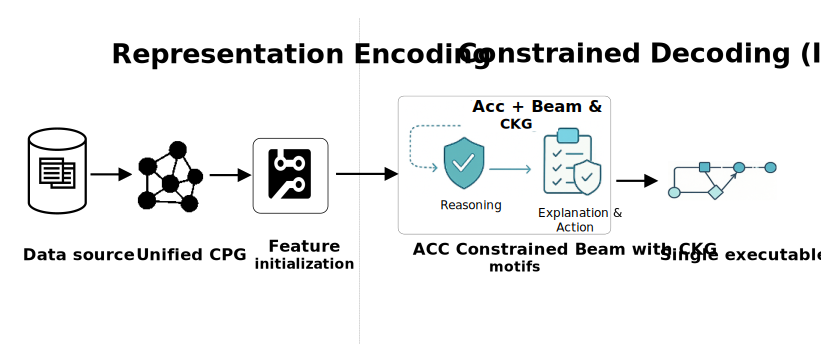
\includegraphics[width=\linewidth]{svg-inkscape/e2e.pdf}
	\caption{Overview of the proposed chain-centric vulnerability analysis approach. Data sources are lifted into a unified CPG) node features are initialized with a pretrained encoder, and an ACC-constrained, CKG-guided beam decoder performs structured reasoning to produce a single executable root-to-sink chain.}
	\label{fig:intro-e2e-pipeline}
\end{figure}


\section{Chain-Centric Program Representation}
\label{sec:chain-conts}

A chain-centric, causal approach to vulnerability detection requires a program representation that explicitly models interprocedural mechanisms. Traditional AST, CFG, DFG, and baseline CPG representations enable local reasoning but lack explicit treatment of root-to-sink propagation paths, which limits executable chain reconstruction across functions, files, and modules. This thesis adopts an augmented CPG that explicitly encodes taint sources, transformations, sanitization, and sinks through control-flow and data-flow, while preserving call/return and aliasing semantics. The representation is designed to be compatible with relation-aware graph encoders and constrained decoding, allowing evidence to propagate along heterogeneous edges and enabling extraction of executable vulnerability chains that support interprocedural causal reasoning.


\subsection{Dataset and Repository Context: ReposVul}
\label{subsec:data-gt}

The chain-centric graphs are derived from \emph{ReposVul}, a repository-level benchmark that links vulnerabilities to concrete pre- and post-fix revisions and retains repository-wide context \cite{wang2024reposvul}. Unlike patch-only corpora, \emph{ReposVul} preserves full file snapshots and cross-file dependencies, which is essential for reconstructing long-range interprocedural flows.

Each \emph{ReposVul} entry links CVE/CWE records to precise pre- and post-fix repository snapshots rather than isolated patches \cite{wang2024reposvul}. A documented weakness and its severity are anchored to the exact commit, preserving all related files and cross-file dependencies. The corpus is constructed by crawling public sources, disentangling mixed commits to isolate fix-relevant code, and extracting caller–callee relations across translation units. By maintaining chronology and repository-wide call structure, \emph{ReposVul} reveals long-range interprocedural flows essential for chain-centric vulnerability analysis. Table~\ref{tab:reposvul-fields} summarises the core metadata captured for each entry, including vulnerability descriptors, patch-level information, and file-level snapshots.


\begin{table}[H]
	\centering
	\small
	\caption{Core metadata recorded per ReposVul entry.}
	\label{tab:reposvul-fields}
	\begin{tabular}{p{0.3\linewidth} p{0.65\linewidth}}
		\toprule
		\textbf{Category} & \textbf{Representative fields} \\
		\midrule
		Vulnerability entry & CVE-ID, CWE-ID, language, external references, CVE description, publish date, CVSS vector (AV, AC, PR, UI, S, C, I, A) \\
		Patch metadata & Commit ID, commit message and date, project/repository IDs, parent/child links, forge URLs \\
		Related files & File name, language, vulnerable/fixed snapshots, line diffs, file URLs \\
		\bottomrule
	\end{tabular}
\end{table}

\subsection{Extraction and Graph Construction Pipeline}
\label{subsec:graph-construction}

The conversion from raw dataset entries to chain-centric program graphs occurs over six sequential stages, as illustrated in Figure~\ref{fig:method-datapipeline}.

\setlength{\fboxsep}{0pt}     
\setlength{\fboxrule}{0.3pt}  
\begin{figure}[H]
	\centering
	\includegraphics[width=\linewidth]{svg-inkscape/datasetpipeline.pdf}
	\caption{ReposVul pipeline: interprocedural CPG construction and leakage-safe data splits.}
	\label{fig:method-datapipeline}
\end{figure}

\paragraph{Stage A: Repository snapshots and vulnerability metadata.}
CVE/CWE metadata is associated with each \emph{ReposVul} entry, and both parent and child commits are retrieved for every patch. Commit identifiers, messages, dates, repository identifiers, and file paths are indexed so that later stages can reconstruct history-aware cross-file context.

\paragraph{Stage B: Normalization and untangling.}
Patches frequently mix vulnerability fixes with unrelated refactorings or vendor code. A corpus untangling rule combining model judgements with static cues is applied to retain only files and hunks that are relevant to the vulnerability fix and to discard unrelated changes.

\paragraph{Stage C: Static graph construction.}
For each retained snapshot, a heterogeneous program graph is built that overlays AST, CFG, and DFG with direct call edges. Pointer and container def–use are approximated by conservative alias relations, identifiers are anonymized, and literals are bucketed to reduce noise from harmless edits \cite{Chakraborty2020,Li2022Empirical}. The result is a chain-ready CPG representation for every project version.

\paragraph{Stage D: Interprocedural augmentation.}
The CPG is enriched with explicit interprocedural edges, including \textsc{CALL}, \textsc{ARG}$\rightarrow$\textsc{PARAM}, and \textsc{RET}$\rightarrow$\textsc{CALLER}/\textsc{RET}$\rightarrow$\textsc{LHS}, together with summary nodes and alias summaries that connect callee summaries back to call sites. This step lifts per-file graphs to repository-level structures that expose long-range flows from candidate sources to potential sinks.

\paragraph{Stage E: Patch-aware differencing and slice materialization.}
Line-level diffs are computed for each patch, and four views are synchronised: changed lines, enclosing functions, touched files, and a reachable repository subgraph that can flow to any sink via control or data edges. 

\paragraph{Stage F: Leakage-safe filtering and splitting.}
File paths, repository identifiers, and commit metadata are used to drop broken files, superseded patches, and obsolete snapshots. The remaining instances are grouped into training, validation, and test sets such that leakage across splits is minimised.

Table~\ref{tab:pipeline} summarises the end-to-end data preparation pipeline, outlining the main stages and their key operations and outputs.

\begin{table}[H]
	\centering
	\caption{Preparation pipeline summary.}
	\label{tab:pipeline}
	\begin{tabular}{p{0.20\linewidth} p{0.75\linewidth}}
		\toprule
		\textbf{Stage} & \textbf{Key operations and outputs} \\
		\midrule
		A & Link CVE/CWE records to parent and child commits; index commits, projects, and file paths. \\
		B & Normalize and untangle patches; keep only fix-relevant files and hunks; deduplicate. \\
		C & Build a heterogeneous CPG per snapshot by overlaying AST, CFG, DFG, and intra-file call edges; anonymize identifiers and bucket literals. \\
		D & Enrich the CPG with interprocedural links (CALL, ARG$\rightarrow$PARAM, RET$\rightarrow$CALLER/RET$\rightarrow$LHS) and alias summaries to expose repository-level flows. \\
		E & Compute line-level diffs; function, file, and reachable-subgraph slices, with rule-based source/flow/stop/sink labels. \\
		F & Drop broken or superseded patches; form leakage-safe train/validation/test splits at the project level. \\
		\bottomrule
	\end{tabular}
\end{table}

\subsection{Unified Multigraph, Typing, Features, and Storage}
\label{subsec:unified-mg}

Each repository snapshot is represented as a heterogeneous multigraph based on the CPG abstraction \cite{yamaguchi2014cpg}. A single typed node store contains program elements (identifiers, literals, statements, basic blocks, functions), and relation-specific edge sets encode \textsc{AST}, \textsc{CFG}, and \textsc{DFG} structure. Interprocedural edges (\textsc{CALL}, \textsc{ARG2PARAM}, \textsc{RET2CALL}, \textsc{RET2LHS}) are materialised in both directions. Graphs are stored in sharded files with repository, commit, and file-path metadata to support scalable provenance and retrieval.

The representation employs a dual-channel feature encoding. A compact structural feature vector captures node type, degree statistics, SSA hints, literal buckets, and role flags, while a 768-dimensional GraphCodeBERT embedding \cite{guo2021graphcodebert} provides contextual token semantics. These two channels are fused during initialization, but the graph topology and interprocedural edge schema remain invariant across variants. The fixed relation alphabet \(\mathcal{R}\) used during message passing and decoding includes all intra- and interprocedural relations exploited by the chain decoder (AST, CFG, DFG, CALL, ARG2PARAM, RET2CALL, RET2LHS, and alias summaries).

\subsection{Ground Truth}
\label{subsec:gt-definition}

Ground truth is defined at two levels. At the revision level, a repository snapshot is labelled vulnerable if it is linked to a corresponding fixed revision in \emph{ReposVul}, which reduces noise from unrelated edits \cite{wang2024reposvul}. At the mechanism level, each positive example carries at least one executable root-to-sink chain that may span multiple functions and files. Sources represent untrusted inputs, sanitizers restrict or reset tainted state, propagators transfer taint through assignments, calls, and returns, and sinks denote security-critical operations. The full role lexicon and matching patterns are listed in Appendix~\ref{app:role-lexicon}.

Chains are seeded from patch diffs, extended along def–use links to identify propagators and candidate sinks, and then wired interprocedurally using \(\textsc{ARG}\!\to\!\textsc{PARAM}\), \(\textsc{RET}\!\to\!\textsc{CALLER}\), and \(\textsc{RET}\!\to\!\textsc{LHS}\) bindings over the call graph. Retained examples satisfy basic consistency criteria: every source reaches at least one sink, every sanitizer blocks at least one tainted path, and every propagator lies on a CFG-consistent route. A feasibility pass verifies that neutralising the sink reduces exploitability, and a counterfactual pass strengthens guards or replaces dangerous sinks with safe ones to confirm that reachability changes as expected. Cases that fail these checks are corrected or discarded.

\medskip
\noindent
Split-wise statistics for the C/C++ subset used in experiments are reported in the experimental setup chapter (Section~\ref{sec:results-setup}).

\section{Model Architecture and Decoding Pipeline}
\label{sec:model-arch}

This section explains how source code and program structure are fused, encoded, and decoded into a single executable chain. All equations and symbol glossaries are consolidated in Appendix~\ref{app:math-model-arch}. Refer to Figure~\ref{fig:model-arch-pipeline} for a comprehensive single-page overview that this section follows.

\setlength{\fboxsep}{0pt}      
\setlength{\fboxrule}{0.3pt}   

\begin{figure}[H]
	\centering
	\includegraphics[width=\linewidth]{svg-inkscape/model_arc.pdf}
	\caption{Chain-Centric Model Architecture and Inference Flow}
	\label{fig:model-arch-pipeline}
\end{figure}

\noindent Node features are initialized with code spans and structural descriptors, encoded via a relation-aware Graph Attention Network (GAT), and decoded into a single executable chain subject to ACC feasibility. Inference begins with seeds selected by the model and can incorporate a Causal Knowledge Graph (CKG) prior for ranking. Training optimizes a composite loss, using CKG derived only from the training split. Solid arrows indicate data or score flow, dashed arrows denote training-only operations, and dotted arrows represent weak decoding priors or optimizer feedback to trainable encoder components. GraphCodeBERT provides pretrained contextual embeddings for code tokens, which are fused with structural descriptors before graph encoding.


\subsection{GraphCodeBERT Feature Initialization}
\label{sec:model-arch-gcbert}

Each node aligned to a concrete source span is tokenized with GraphCodeBERT’s byte-pair encoding and encoded in sliding windows (length $L$, stride $S$). Window-level contextual token embeddings are aggregated back to the node: if the span contains identifiers, a light edge-aware attention emphasizes tokens carrying def–use signal (Appendix Eqs.~\ref{app:eq:gcbert-attn-weight}--\ref{app:eq:gcbert-attn-sum}); otherwise a simple average is used (Appendix Eq.~\ref{app:eq:gcbert-token-avg}). Spans that appear in multiple windows are pooled per window and then averaged, and function-proxy nodes pool their child statements to obtain a coarse function representation.

The textual embedding $\mathbf{x}^{\text{text}}_i$ and structural descriptor $\mathbf{x}^{\text{struct}}_i$ (node type, degrees, SSA hints, literal statistics, role flags) are both projected to dimension $d_0$ and fused via a learned gating mechanism to obtain the initial node state $\mathbf{h}^{(0)}_i$ (Appendix Eqs.~\ref{app:eq:init-proj}--\ref{app:eq:init-fuse}). When a node and its def–use neighbours fall within a single window, GraphCodeBERT’s data-flow mask is enabled so these pairs can attend directly; the encoder remains frozen to attribute performance gains to the graph module, and Table~\ref{tab:feat-dims} summarizes the resulting feature dimensionalities.


\begin{table}[H]
	\centering
	\caption{Node feature dimensions at initialization.}
	\label{tab:feat-dims}
	\begin{tabular}{lrl}
		\toprule
		\textbf{Component} & \textbf{Dim.} & \textbf{Notes} \\
		\midrule
		Textual embedding & 768 & GraphCodeBERT contextual vector \cite{guo2021graphcodebert} \\
		Structural raw & 100–200 & Type, role, degree, SSA hint, literal buckets \\
		Projected text & $d_0$ & $W_t:\mathbb{R}^{768}\!\to\!\mathbb{R}^{d_0}$ (with LN) \\
		Projected structural & $d_0$ & $W_s:\mathbb{R}^{d_s}\!\to\!\mathbb{R}^{d_0}$ (with LN) \\
		Fused node init $h^{(0)}$ & $d_0$ & Gated combination for the GAT encoder \\
		\bottomrule
	\end{tabular}
\end{table}


\subsection{GAT with Causality\texorpdfstring{-}{-}Oriented Attention}
\label{sec:model-arch-gat}
A relation-aware Graph Attention Network consumes the fused initializations and builds contextual node states while learning how different edge types contribute to aggregation. Per layer, attention and updates follow Appendix Eqs.~\ref{app:eq:gat-alpha}–\ref{app:eq:gat-update}. After $L$ layers the encoder emits a node vulnerability logit $z_v$, a seed score $s_v$, and relation-gated edge compatibilities $c^{(r)}_{u\to v}$ (Appendix Eqs.~\ref{app:eq:node-seed}–\ref{app:eq:edge-compat}). Seeds identify likely chain starts as the top-$K$ nodes by $s_v$ (Appendix Eq.~\ref{app:eq:seed-set}); candidate paths are scored by a log-additive mixture of node evidence and edge compatibility (Appendix Eq.~\ref{app:eq:path-score}), with $\alpha$ controlling the mix. Training couples node- and edge-level objectives with a path-margin term so that true chains outrank admissible distractor walks.


\subsection{Causal Knowledge Graph (CKG): Mining and Prior}
\label{sec:model-arch-ckg}
From training chains only, unigram and bigram statistics are mined over the relation alphabet. At decoding time, admissibility is unchanged, but the ranking of admissible expansions receives a small prior bonus $S_{\mathrm{CKG}}(\pi)$ mixed into the path score with weight $\lambda$ (Appendix Eq.~\ref{app:eq:path-score-ckg}). This preserves data-driven evidence while gently preferring historically plausible relation patterns. 


\subsection{Adaptive Causal Contextualization (ACC)}
\label{sec:model-arch-acc}
ACC converts encoder scores into a single executable interprocedural chain by enforcing constant-time feasibility checks and role-shaped preferences. A partial path maintains a taint footprint, a call stack, and accumulated guards; an expansion $u\xrightarrow{r}v$ is admissible only if all predicates hold (Appendix Eqs.~\ref{app:eq:acc-cfg-ok}–\ref{app:eq:acc-admiss}). The path score is adjusted by start/middle/end role penalties and a sanitizer dominance bonus (Appendix Eqs.~\ref{app:eq:acc-role-start}–\ref{app:eq:acc-san-bonus}), together with mild length and repetition costs (Appendix Eqs.~\ref{app:eq:acc-pen-len}–\ref{app:eq:acc-pen-rep}), yielding the ACC objective $S_{\mathrm{ACC}}(\pi)$ and its optional CKG mixture $S_{\mathrm{ACC}}^{\star}(\pi)$ (Appendix Eqs.~\ref{app:eq:acc-score}–\ref{app:eq:acc-score-ckg}). On \texttt{CALL}, the callee and site are pushed; \texttt{RET2CALL}/\texttt{RET2LHS} pop only with matching sites, preserving well-nested cross-function paths. The decoding complexity with beam width $B$, horizon $H$, and average admissible out-degree $\bar{d}$ scales as $\mathcal{O}(B \cdot H \cdot \bar{d})$. This reflects exploring $B$ candidates over $H$ steps, each with $\bar{d}$ possible expansions, consistent with standard beam search computational cost analyses.

\subsection{Chain Extraction and Validation}
\label{sec:model-arch-extract-validate}
A candidate is valid if it starts near a source, contains at least one interior propagator or sanitizer, and ends at a sink (Appendix Eqs.~\ref{app:eq:chain-start}–\ref{app:eq:chain-end}); when interprocedural links exist in the slice, at least one must appear in the chain. Among admissible paths across beams from the top-$K$ seeds, selection maximizes $S_{\mathrm{ACC}}(\pi)$ (Appendix Eq.~\ref{app:eq:chain-select}). The final chain is then validated structurally and counterfactually.

\subsection{Training, Optimization, and Hyperparameters}
\label{sec:method-train}
The total loss combines graph-level binary cross-entropy with regularizers for flow and counterfactual consistency, attention entropy, spectral control, and sanitizer alignment. The CKG prior is applied only at decoding time. Models are trained with AdamW, cosine learning-rate decay, gradient clipping, mixed precision, and weighted sampling for class imbalance. Semantics-preserving augmentations (renaming, benign reordering) are used, and fixed seeds, logged checkpoints, cached features, and archived training curves support reproducibility.

This chapter summarizes a five-step methodology for reconstructing executable root-to-sink vulnerability chains. First, nodes are encoded with GraphCodeBERT and fused with structural features to obtain context-sensitive initial states for all program elements (Appendix Eqs.~\ref{app:eq:gcbert-attn-weight}–\ref{app:eq:init-fuse}). Second, a relation-aware graph attention network propagates information along heterogeneous control-, data-, and call/return edges so that node representations reflect their interprocedural context (Appendix Eqs.~\ref{app:eq:gat-alpha}–\ref{app:eq:gat-update}). Third, a constrained decoder guided by a weak causal knowledge graph prior scores and assembles candidate paths, restricting search to syntactically and semantically plausible root-to-sink sequences (Appendix Eq.~\ref{app:eq:path-score-ckg}). Fourth, adaptive causal contextualization (ACC) filters and selects chains that satisfy control-flow, data-flow, and aliasing constraints, ensuring that only semantically valid mechanisms are retained (Appendix Eqs.~\ref{app:eq:acc-cfg-ok}–\ref{app:eq:chain-select}). Finally, the entire model is trained at the graph level using binary cross-entropy loss with light regularization (Appendix Eq.~\ref{app:eq:train-total}), aligning vulnerability predictions with the reconstructed executable chains.


\chapter{Experimental Results and Analysis}
\label{chap:results}

This chapter presents the experimental results for the proposed chain-centric interprocedural vulnerability detector. Under the default \texttt{ReposVul} splits, it quantifies graph-level detection performance, the quality of reconstructed root–propagation–sink chains, causal consistency under targeted interventions, and inference cost and decoding behaviour. All results are obtained under a single, leakage-safe experimental setup and are averaged over five seeds to support reproducibility.

The analysis progresses from an overview of global behaviour to a detailed mechanism-level examination. It first summarises the dataset, model variants, and evaluation metrics used throughout the experiments, then presents detection metrics for both encoder configurations. Subsequent sections examine executable chain feasibility and interprocedural structure, evaluate causal faithfulness via counterfactual edits, and characterise decoding efficiency. The chapter concludes with robustness experiments and a case study that illustrates how an executable root–propagation–sink chain is reconstructed on a real test instance.

\section{Experimental Setup and Configuration}
\label{sec:results-setup}

This section summarizes the experimental setup used throughout the evaluation, including datasets and default splits.

\medskip
\noindent\textbf{Dataset and splits:}
All experiments use the default splits provided with \texttt{ReposVul}~\cite{wang2024reposvul}. Splits are repository-disjoint, so code from the same repository does not appear in multiple splits. Positive and negative pairs are kept within the same split, and, when reported, chronology is respected so that training data does not depend on future revisions. 

Tables~\ref{tab:split-labels}–\ref{tab:ipa-coverage} report split-wise statistics for the prepared C and C++ subset used in the experiments, including label balance at the file-snapshot level, graph and node-label density after chain-centric conversion, and the prevalence of interprocedural caller/callee structure.

\begin{table}[H]
	\centering
	\small
	\caption{File-level label counts by split (C/C++ subset).}
	\label{tab:split-labels}
	\begin{tabular}{lrrrr}
		\toprule
		\textbf{Split} & \textbf{Records} & \textbf{Non-vuln} & \textbf{Vuln} & \textbf{Pos.\%} \\
		\midrule
		Train & 185{,}791 & 180{,}259 & 5{,}532 & 2.98 \\
		Valid & 23{,}224 & 22{,}503 & 721 & 3.10 \\
		Test  & 23{,}224 & 22{,}554 & 670 & 2.88 \\
		\bottomrule
	\end{tabular}
\end{table}

\begin{table}[H]
	\centering
	\small
	\caption{Graph instances and node-label density after chain-centric conversion.}
	\label{tab:graph-density}
	\begin{tabular}{lrrrr}
		\toprule
		\textbf{Split} & \textbf{Graphs} & \textbf{Vuln nodes} & \textbf{Non-vuln nodes} & \textbf{Pos.\ ratio} \\
		\midrule
		Train & 3{,}438 & 9{,}946 & 25{,}173{,}258 & $3.95\times10^{-4}$ \\
		Valid & 2{,}905 & 1{,}455 & 3{,}970{,}281 & $3.66\times10^{-4}$ \\
		Test  & 2{,}915 & 1{,}316 & 3{,}973{,}974 & $3.31\times10^{-4}$ \\
		\bottomrule
	\end{tabular}
\end{table}

\begin{table}[H]
	\centering
	\small
	\caption{Interprocedural connectivity (non-empty caller and callee sets).}
	\label{tab:ipa-coverage}
	\begin{tabular}{lrrrrrr}
		\toprule
		\textbf{Split} & \textbf{Caller\%} & \textbf{Callee\%} & \textbf{Both\%} & \textbf{Caller\_chg\%} & \textbf{Callee\_chg\%} & \textbf{Both\_chg\%} \\
		\midrule
		Train & 12.59 & 28.95 & 8.72 & 0.46 & 2.79 & 0.06 \\
		Valid & 13.10 & 29.26 & 9.21 & 0.55 & 2.74 & 0.07 \\
		Test  & 12.97 & 29.17 & 9.03 & 0.47 & 2.90 & 0.09 \\
		\bottomrule
	\end{tabular}
\end{table}

\noindent
These statistics indicate that roughly one third of instances have at least one callee, about one eighth have at least one caller, and around one tenth have both, providing the minimal interprocedural structure required to reconstruct vulnerability chains that span function boundaries.


\medskip
\noindent\textbf{Inputs and graph relations:}
Models operate on chain-prepared interprocedural CPGs that overlay ASTs, CFGs, and DFGs, and include interprocedural relations \texttt{CALL}, \texttt{ARG}$\!\to$\texttt{PARAM}, \texttt{RET}$\!\to$\texttt{CALLER}/\texttt{RET}$\!\to$\texttt{LHS}, together with alias summaries. Table~\ref{tab:results-config} summarizes the main graph, encoder, decoding, training, and calibration settings shared across all experiments.

\begin{table}[H]
	\centering
	\small
	\setlength{\tabcolsep}{6pt}
	\renewcommand{\arraystretch}{1.06}
	\caption{Experimental Setup Details.}
	\label{tab:results-config}
	\begin{tabularx}{\linewidth}{@{} l X @{}}
		\toprule
		\textbf{Item} & \textbf{Setting} \\
		\midrule
		Dataset & \texttt{ReposVul}, default repository-disjoint splits, chronology respected \\
		Graph relations & DFG, CFG, CALL, ARG2PARAM, RET2CALL, RET2LHS; alias summaries enabled \\
		Encoder & Relation-aware GAT, width \(d_0{=}64\), \(L{=}3\) layers \\
		Variants & Struct-only; GCBERT+Struct (GraphCodeBERT frozen) \\
		Decoding & Beam with ACC, \(K{=}8\), \(B{=}24\), \(H{=}5\), node/edge mix \(\alpha{=}0.7\) \\
		CKG prior & Decoding-only mixture \(\lambda{=}0.2\); smoothing \(10^{-3}\); temperature \(1.0\) \\
		Training & AdamW; LR \(2\times10^{-3}\); WD \(10^{-4}\); early stop on validation macro-F1 \\
		Calibration & Temperature scaling on validation; ECE with 15 bins \\
		Thresholds & \(\tau_{\mathrm{F1}^\star}\) (per variant) and \(\tau{=}0.5\) \\
		Seeds & 5 per configuration; mean and 95\% CIs reported \\
		Environment & PyTorch 2.4.1, CUDA 12.1, RTX 4070 Laptop GPU, AMP on \\
		Embeddings cache & GraphCodeBERT features, FP16, max length 512, stride 384 \\
		\bottomrule
	\end{tabularx}
\end{table}

\noindent\textbf{Model variants:}
Two encoder configurations are compared under the same graph topology and training/decoding regime. The \emph{Struct-only} variant uses compact structural features (types, degrees, SSA hints, literal buckets), while \emph{GCBERT+Struct} augments these with frozen GraphCodeBERT embeddings~\cite{guo2021graphcodebert}. Table~\ref{tab:gcbert-topology} contrasts the resulting graph topology and feature dimensionality on a representative shard.

\begin{table}[H]
	\centering
	\small
	\setlength{\tabcolsep}{4pt}
	\renewcommand{\arraystretch}{1.05}
	\caption{Comparison of Struct-only vs.\ GCBERT+Struct encodings.}
	\label{tab:gcbert-topology}
	\resizebox{\linewidth}{!}{%
		\begin{tabular}{llll}
			\toprule
			\textbf{Property} & \textbf{Struct-only} & \textbf{GCBERT} & \textbf{Comment} \\
			\midrule
			Nodes / in-dim & 3141 / 25  & 3141 / 793 & \(25{+}768\) features in GCBERT \\
			Total edges    & 14066       & 14066      & Unchanged \\
			Interproc edges (sum) & 4818  & 4818       & CALL/ARG2PARAM/RET2* identical \\
			Feature memory (approx.) & \(\sim 0.31\) MB & \(\sim 9.50\) MB & Text channel dominates \\
			\bottomrule
		\end{tabular}%
	}
\end{table}

\noindent\textbf{Decoding and evaluation:}
Decoding uses ACC-constrained beam search, allowing only moves that satisfy control-flow reachability, consistent ARG$\to$PARAM and RET$\to$CALLER/LHS bindings, alias checks, and stack discipline. A causal knowledge graph (CKG) prior mined from training chains adjusts move scores during inference but does not alter admissibility. Training uses class-weighted binary cross-entropy at the graph level with flow and causal regularizers, early stopping on validation macro-F1, and calibrated thresholds derived from validation data. Table~\ref{tab:eval-configuration} summarizes the decoding, training, and evaluation configuration.

\begin{table}[H]
	\centering
	\small
	\setlength{\tabcolsep}{6pt}
	\renewcommand{\arraystretch}{1.06}
	\caption{Decoding and Training Configuration.}
	\label{tab:eval-configuration}
	\begin{tabularx}{\linewidth}{@{} l X @{}}
		\toprule
		\textbf{Item} & \textbf{Setting} \\
		\midrule
		Beam / horizon / mix & $K{=}8$, $B{=}24$, $H{=}5$, node–edge mix $\alpha{=}0.7$ \\
		Admissibility gates & CFG reachability, ARG$\to$PARAM, RET$\to$CALLER/LHS, alias checks, stack discipline \\
		CKG prior (inference only) & Mixture $\lambda{=}0.2$; smoothing $\epsilon{=}10^{-3}$; temperature $\tau{=}1.0$; top-$K$ trigrams $=500$; weights $(\beta_1,\beta_2,\beta_3){=}(0.3,0.6,0.1)$ \\
		Loss & Class-weighted BCE at graph level $+$ flow and causal regularizers \\
		Early stopping & Macro-F1 on validation, patience $=5$ \\
		Encoder freeze & GraphCodeBERT frozen; ablation unfreezes last 2 blocks at $0.1\times$ LR \\
		Thresholds & $\tau_{\text{F1}^\star}$ from validation and fixed $\tau{=}0.5$ on test \\
		Calibration & Temperature scaling fit on validation; ECE with 15 bins \\
		Seeds \& uncertainty & 5 seeds; mean and 95\% CIs; bootstrap $10^4$ for metrics, binomial CIs for DCR, paired bootstrap with Cliff’s $\delta$ \\
		\bottomrule
	\end{tabularx}
\end{table}

\noindent\textbf{Experiment Environment and Artifact:}
\label{subsec:results-env}
Experiments were run on an NVIDIA RTX 4070 Laptop GPU with CUDA 12.1 and PyTorch 2.4.1 using automatic mixed precision. GraphCodeBERT embeddings were precomputed and cached as FP16 tensors. The artifact archive includes configuration files, predictions, calibration parameters, causal intervention logs, beam expansion analyses, and environment metadata. This setup ensures full reproducibility of the results, with all decoding, calibration, and reporting details preserved.

\section{Evaluation Metrics}
\label{sec:eval-metrics}
This section defines the standard classification, chain-centric, and counterfactual metrics used to assess detection performance, executable chain quality, and causal faithfulness of the proposed approach.

\subsection{Standard Classification Metrics}
\label{sec:eval-std}

Classification models are commonly evaluated by thresholding predicted probabilities to produce discrete labels, enabling the construction of a confusion matrix from counts of true positives (TP), false positives (FP), true negatives (TN), and false negatives (FN). From these counts, primary metrics such as Precision, Recall, and F1 score are computed:
\begin{equation}
	\label{eq:prf1}
	\mathrm{Precision}=\frac{\mathrm{TP}}{\mathrm{TP}+\mathrm{FP}},\quad
	\mathrm{Recall}=\frac{\mathrm{TP}}{\mathrm{TP}+\mathrm{FN}},\quad
	\mathrm{F1}=\frac{2\,\mathrm{Precision}\cdot \mathrm{Recall}}{\mathrm{Precision}+\mathrm{Recall}}.
\end{equation}
Precision quantifies the accuracy of positive predictions, Recall measures the coverage of actual positives, and F1 balances the two in a single harmonic mean. Additionally, metrics including Accuracy, Macro-/Micro-F1, AUROC, and AUPRC are computed on the raw prediction scores without thresholding. Due to the low prevalence of vulnerable instances, AUPRC and Macro-F1 are emphasized as primary indicators of detection performance. Formal definitions are detailed in Appendix~\ref{app:metrics-standard}.


\subsection{Chain-Centric Metrics}
\label{sec:eval-chain}

For each positive decision, at most one executable chain is returned (or none if feasibility is not met).
\medskip

\noindent\textbf{Validity:} The fraction of returned chains that satisfy ACC feasibility checks is reported. These checks include CFG reachability, def–use or guard consistency, interprocedural call–return discipline, and alias coherence. The formal definition is in Appendix.~\ref{app:eq-validity}.

\noindent\textbf{Structural fidelity:} When a reference chain is available, reported metrics include node and edge coverage, longest common subsequence ratio (LCS), and role-aware coverage for {source, sanitizer, propagator, sink}. Formulas are detailed in Appendix~\ref{app:eq-struct}.

\noindent\textbf{Interprocedurality:} The IPA Rate quantifies the share of predicted chains that traverse \texttt{CALL}/\texttt{ARG}$\!\to$\texttt{PARAM}/\texttt{RET} edges when such edges exist in the slice (Appendix.~\ref{app:eq-ipa}).

\subsection{Counterfactual Metrics}
\label{sec:eval-cf}

Causal robustness is evaluated through three targeted interventions: guard strengthening, call unbinding, and sink neutralization. Results are reported by intervention type with confidence intervals; detailed methods are provided in Appendices~\ref{app:eq-ccs} and~\ref{app:eq-cfam}. The CKG prior is active except during robustness tests, when it is disabled on the edited graph.

\medskip
\noindent\textbf{Counterfactual Consistency Score (CCS):}
\begin{equation}
	\label{eq:ccs}
	\mathrm{CCS}_i = (p_i - p_i^{\mathrm{do}})^2,
\end{equation}
where \(p_i\) and \(p_i^{\mathrm{do}}\) denote the predicted probabilities before and after the targeted intervention on graph \(i\), respectively, both bounded in \([0,1]\). A low CCS indicates minimal change in prediction, while a high CCS signals a substantial effect of the intervention. Appendix~\ref{app:eq-ccs} further defines a directional consistency rate assessing whether changes occur in the expected direction per intervention type.

\medskip
\noindent\textbf{Causal Feature Attribution Measure (CFAM):}
\begin{equation}
	\label{eq:cfam}
	\mathrm{CFAM}_i = \frac{\sum_{f \in F_c} A_i(f)}{\sum_{f \in F_c \cup F_s} A_i(f)} \in [0,1],
\end{equation}
where \(F_c\) and \(F_s\) are sets of on-chain and off-chain features, respectively, and \(A_i(f) \geq 0\) denotes the attribution score of feature \(f\) in graph \(i\). CFAM quantifies the fraction of total attribution attributed to features on the returned causal chain. Values near 1 indicate strong alignment of attribution with the chain's features. Normalization details are given in Appendix~\ref{app:eq-cfam}. Auxiliary decoding diagnostics, including Chain Success Rate, admissible expansion ratio, and prior influence rate, are defined in Appendix~\ref{app:metrics-diag}.

\section{Detection Results}
\label{sec:results-conventional}

For both encoder variants, this section reports standard graph-level metrics: Accuracy, Precision, Recall, F1, AUROC, and AUPRC. The operating threshold \(\tau_{\text{F1}^\star}\) is selected on the validation split and applied unchanged to the test set. Probabilities are calibrated via temperature scaling on validation and reused on test, and calibration quality is summarised using Expected Calibration Error (ECE), where lower values indicate better alignment between predicted confidence and empirical accuracy (formal definition and binning scheme in Appendix~\ref{app:eq-ece}). AUPRC is treated as the primary metric, with F1 and AUROC providing additional context given the class imbalance in the test set (positives \(\approx 2.9\%\)). All results are averaged over five random seeds.

Table~\ref{tab:conv-metrics} reports validation and test performance at \(\tau_{\text{F1}^\star}\) (mean over five seeds) for both encoder variants, including thresholded Accuracy, Precision, Recall, F1, and the corresponding AUROC and AUPRC values.

\begin{table}[H]
	\centering
	\small
	\caption{Valid and test metrics for Struct-only and GCBERT+Struct.}
	\label{tab:conv-metrics}
	\begin{tabular}{l l c c c c c}
		\toprule
		Split & Variant & Acc & Prec & Rec & F1 & AUROC / AUPRC \\[1pt]
		\midrule
		Valid & Struct-only      & 0.954 & 0.320 & 0.530 & 0.400 & 0.820 / 0.300 \\
		Valid & GCBERT+Struct    & 0.963 & 0.450 & 0.660 & 0.540 & 0.890 / 0.450 \\
		\midrule
		Test  & Struct-only      & 0.953 & 0.310 & 0.520 & 0.390 & 0.810 / 0.280 \\
		Test  & GCBERT+Struct    & 0.965 & 0.440 & 0.640 & 0.520 & 0.880 / 0.430 \\
		\bottomrule
	\end{tabular}
\end{table}

Across both valid and test splits, the GCBERT+Struct configuration yields higher F1 and AUPRC than Struct-only (AUPRC \(+0.15\), F1 \(+0.14\) on \textsc{Valid}; AUPRC \(+0.15\), F1 \(+0.13\) on \textsc{Test}). Accuracy remains high for both variants due to class imbalance, while AUROC indicates stable ranking performance.

Table~\ref{tab:conv-thresh} summarises the corresponding operating thresholds and calibration parameters, including the learned temperature \(T\) and ECE values before and after temperature scaling.

\begin{table}[H]
	\centering
	\small
	\caption{Operating thresholds and calibration parameters.}
	\label{tab:conv-thresh}
	\begin{tabular}{l l c c c c}
		\toprule
		Split & Variant & \(\tau_{\text{F1}^\star}\) & Temp \(T\) & ECE (before) & ECE (after) \\[1pt]
		\midrule
		Valid & Struct-only      & 0.32 & 1.41 & 0.079 & 0.034 \\
		Valid & GCBERT+Struct    & 0.27 & 1.29 & 0.061 & 0.021 \\
		\midrule
		Test  & Struct-only      & 0.32 & 1.41 & 0.082 & 0.036 \\
		Test  & GCBERT+Struct    & 0.27 & 1.29 & 0.064 & 0.022 \\
		\bottomrule
	\end{tabular}
\end{table}

Calibration reduces ECE for both variants, and the relative ordering between Struct-only and GCBERT+Struct is consistent with the improvements observed in AUPRC and F1. Precision–Recall and ROC curves exhibit the same pattern. To contextualise these aggregate metrics, Table~\ref{tab:cm-both} presents confusion matrices on \textsc{Test} at \(\tau_{\text{F1}^\star}\) for both encoder variants.

\begin{table}[H]
	\centering
	\small
	\caption{Confusion matrices on \textsc{Test} at \(\tau_{\text{F1}^\star}\) for Struct-only and GCBERT+Struct.}
	\label{tab:cm-both}
	\begin{tabular}{l rr rr}
		\toprule
		& \multicolumn{2}{c}{Struct-only} & \multicolumn{2}{c}{GCBERT+Struct} \\
		\cmidrule(lr){2-3}\cmidrule(lr){4-5}
		& Pred.\ Neg & Pred.\ Pos & Pred.\ Neg & Pred.\ Pos \\
		\midrule
		True Neg & 21{,}779 & 775 & 22{,}008 & 546 \\
		True Pos & 322 & 348 & 241 & 429 \\
		\bottomrule
	\end{tabular}
\end{table}

False positives correspond to safe code incorrectly flagged as vulnerable, while false negatives indicate missed vulnerabilities. In this setting, many false negatives arise in macro-expanded code or callback-driven execution paths, where control flow is implicit and interprocedural structure is more difficult to recover faithfully.


\section{Executable Chain Quality and Interprocedural Evidence}
\label{sec:results-chain-quality}

This section evaluates the quality of reconstructed chains using feasibility, interprocedural usage, structural agreement with ground truth, and chain length/span statistics. All quantities are computed on positive slices and averaged over five seeds. Table~\ref{tab:validity} reports the fraction of predicted chains that pass all ACC feasibility checks (control-flow reachability, call/return consistency, data/guard preservation, alias coherence).

\begin{table}[H]
	\centering
	\small
	\setlength{\tabcolsep}{8pt}
	\renewcommand{\arraystretch}{1.10}
	\caption{Feasibility of reconstructed chains (pass of all checks).}
	\label{tab:validity}
	\begin{tabular}{l l c c}
		\toprule
		\textbf{Split} & \textbf{Variant} & \textbf{Validity} & \textbf{Notes} \\
		\midrule
		Valid & Struct-only      & 0.762 & More CFG violations in long hops \\
		Valid & GCBERT+Struct    & 0.842 & Fewer alias/stack failures \\
		Test  & Struct-only      & 0.741 & Errors concentrate at returns \\
		Test  & GCBERT+Struct    & 0.823 & Higher pass rate across seeds \\
		\bottomrule
	\end{tabular}
\end{table}

\noindent
GCBERT+Struct improves chain feasibility on both validation and test splits. Table~\ref{tab:ipa} summarizes interprocedural usage: the IPA rate (share of chains that use any CALL/ARG$\to$PARAM/RET edges), the fraction that include both call and return edges, and the mean call depth.

\begin{table}[H]
	\centering
	\small
	\setlength{\tabcolsep}{6pt}
	\renewcommand{\arraystretch}{1.10}
	\caption{Interprocedural structure in predicted chains.}
	\label{tab:ipa}
	\begin{tabular}{l l c c c}
		\toprule
		\textbf{Split} & \textbf{Variant} & \textbf{IPA rate} & \textbf{Both(call+ret)} & \textbf{Mean call depth} \\
		\midrule
		Valid & Struct-only      & 0.618 & 0.402 & 1.27 \\
		Valid & GCBERT+Struct    & 0.708 & 0.486 & 1.32 \\
		Test  & Struct-only      & 0.603 & 0.389 & 1.24 \\
		Test  & GCBERT+Struct    & 0.691 & 0.471 & 1.30 \\
		\bottomrule
	\end{tabular}
\end{table}

\noindent
The enriched encoder yields higher IPA rates, more chains that use both call and return edges, and slightly deeper call stacks.

Table~\ref{tab:role-order} reports node and edge coverage, together with role-aware coverage for \emph{source}, \emph{sanitizer}, \emph{propagator}, and \emph{sink} nodes against the reference chains, and Table~\ref{tab:lcs} summarises order agreement using the longest common subsequence (LCS) ratio.


\begin{table}[H]
	\centering
	\small
	\setlength{\tabcolsep}{1pt}
	\renewcommand{\arraystretch}{1.12}
	\caption{Role and edge agreement with ground truth.}
	\label{tab:role-order}
	\resizebox{\linewidth}{!}{%
		\begin{tabular}{l l c c c c c c}
			\toprule
			\textbf{Split} & \textbf{Variant} & \textbf{NodeCov} & \textbf{EdgeCov} & \textbf{RoleCov\_src} & \textbf{RoleCov\_san} & \textbf{RoleCov\_prop} & \textbf{RoleCov\_sink} \\
			\midrule
			Valid & Struct-only      & 0.583 & 0.462 & 0.781 & 0.412 & 0.551 & 0.692 \\
			Valid & GCBERT+Struct    & 0.671 & 0.552 & 0.842 & 0.521 & 0.619 & 0.763 \\
			Test  & Struct-only      & 0.571 & 0.451 & 0.773 & 0.398 & 0.542 & 0.681 \\
			Test  & GCBERT+Struct    & 0.658 & 0.540 & 0.834 & 0.507 & 0.607 & 0.752 \\
			\bottomrule
		\end{tabular}%
	}
\end{table}


\begin{table}[H]
	\centering
	\small
	\setlength{\tabcolsep}{10pt}
	\renewcommand{\arraystretch}{1.10}
	\caption{Order agreement via LCS ratio.}
	\label{tab:lcs}
	\begin{tabular}{l l c c}
		\toprule
		\textbf{Split} & \textbf{Variant} & \textbf{LCS ratio} & \textbf{Comment} \\
		\midrule
		Valid & Struct-only      & 0.523 & Mismatches at call boundaries \\
		Valid & GCBERT+Struct    & 0.604 & Better call/return placement \\
		Test  & Struct-only      & 0.515 & Early sink hops reduce LCS \\
		Test  & GCBERT+Struct    & 0.595 & More faithful step order \\
		\bottomrule
	\end{tabular}
\end{table}

\noindent
GCBERT+Struct improves both coverage (especially for sanitizers and propagators) and order agreement. Finally, Table~\ref{tab:chain-length-span} characterises chain length and span via hop count, number of files crossed, and the proportion of summary edges.

\begin{table}[H]
	\centering
	\small
	\setlength{\tabcolsep}{8pt}
	\renewcommand{\arraystretch}{1.10}
	\caption{Chain length and span: hops, files crossed, and summary-edge share.}
	\label{tab:chain-length-span}
	\resizebox{\linewidth}{!}{%
		\begin{tabular}{l l c c c c}
			\toprule
			\textbf{Split} & \textbf{Variant} & \textbf{Mean hops} & \textbf{Median} & \textbf{Files crossed} & \textbf{Summary-edge share} \\
			\midrule
			Valid & Struct-only      & 4.70 & 4 & 1.57 & 0.18 \\
			Valid & GCBERT+Struct    & 4.52 & 4 & 1.49 & 0.12 \\
			Test  & Struct-only      & 4.66 & 4 & 1.55 & 0.17 \\
			Test  & GCBERT+Struct    & 4.48 & 4 & 1.47 & 0.12 \\
			\bottomrule
		\end{tabular}%
	}
\end{table}

\noindent
Chains remain short and typically span one to two files, with similar hop counts across variants. The enriched encoder slightly reduces reliance on summary edges while increasing feasibility, interprocedural usage, and agreement with ground-truth chains.

\section{Causal Faithfulness}
\label{sec:res-causal}

This section evaluates how strongly predictions depend on the reconstructed chains using counterfactual interventions. The \emph{Counterfactual Consistency Score} (CCS) measures the magnitude of probability changes under edits, the \emph{Directional Consistency Rate} (DCR) captures how often changes move in the expected direction, the \emph{Causal Feature Attribution Measure} (CFAM) quantifies how much attribution mass lies on the predicted chain, and the chain invalidation rate records how often no valid chain remains after editing. Formal definitions and variants are given in Appendix~\ref{app:eq-ccs} and Appendix~\ref{app:eq-cfam}.

Table~\ref{tab:cf-proto} reports prototype CCS and CFAM values averaged over a small subset of graphs, illustrating the scale of probability shifts and on-chain attribution at different training stages.

\begin{table}[H]
	\centering
	\small
	\setlength{\tabcolsep}{8pt}
	\renewcommand{\arraystretch}{1.06}
	\caption{Prototype causal metrics (means over $N{=}256$ graphs per split).}
	\label{tab:cf-proto}
	\begin{tabular}{lccc}
		\toprule
		\textbf{Split} & \textbf{CCS (mean)} & \textbf{CFAM (mean)} & \textbf{Notes} \\
		\midrule
		Train & $1.76\!\times\!10^{-9}$ & $0.0047$ & Early-epoch snapshot \\
		Valid & $8.89\!\times\!10^{-9}$ & $0.0232$ & Default $\tau{=}0.25$ \\
		Test  & $7.97\!\times\!10^{-9}$ & $0.0233$ & Same thresholding \\
		\bottomrule
	\end{tabular}
\end{table}

Table~\ref{tab:cf-ccs-edits} decomposes CCS by intervention type: strengthening guards and unbinding calls (minor edits) versus sink neutralisation (major edit). Minor edits produce small probability shifts, while sink edits cause substantially larger changes, indicating that the endpoint of the chain has strong influence on the decision.

\begin{table}[H]
	\centering
	\small
	\setlength{\tabcolsep}{6pt}
	\renewcommand{\arraystretch}{1.06}
	\caption{CCS by edit type (lower is better for minor, higher for sink edits).}
	\label{tab:cf-ccs-edits}
	\begin{tabular}{l l r r r}
		\toprule
		\textbf{Split} & \textbf{Variant} & \textbf{Guard (minor)} & \textbf{Unbind (minor)} & \textbf{Sink (major)} \\
		\midrule
		Valid & Struct-only      & 0.0048 & 0.0112 & 0.118 \\
		Valid & GCBERT+Struct    & 0.0039 & 0.0091 & 0.134 \\
		Test  & Struct-only      & 0.0051 & 0.0120 & 0.112 \\
		Test  & GCBERT+Struct    & 0.0041 & 0.0098 & 0.129 \\
		\bottomrule
	\end{tabular}
\end{table}

Table~\ref{tab:cf-dcr} shows the Directional Consistency Rate (DCR), that is, the proportion of edits where the probability change has the expected sign. DCR is high for all edits, particularly for sink interventions, indicating stable qualitative responses to causal perturbations.

\begin{table}[H]
	\centering
	\small
	\setlength{\tabcolsep}{6pt}
	\renewcommand{\arraystretch}{1.06}
	\caption{Directional consistency rate (DCR; higher is better).}
	\label{tab:cf-dcr}
	\begin{tabular}{l l r r r}
		\toprule
		\textbf{Split} & \textbf{Variant} & \textbf{Guard} & \textbf{Unbind} & \textbf{Sink} \\
		\midrule
		Valid & Struct-only      & 0.78 & 0.81 & 0.93 \\
		Valid & GCBERT+Struct    & 0.82 & 0.85 & 0.95 \\
		Test  & Struct-only      & 0.76 & 0.79 & 0.91 \\
		Test  & GCBERT+Struct    & 0.81 & 0.83 & 0.94 \\
		\bottomrule
	\end{tabular}
\end{table}

Table~\ref{tab:cf-cfam-role} presents CFAM scores overall and decomposed by chain segment (source, sanitizer, propagator, sink), with values in \([0,1]\). Higher values indicate that a larger share of attribution mass lies on nodes that belong to the returned chain.

\begin{table}[H]
	\centering
	\small
	\setlength{\tabcolsep}{6pt}
	\renewcommand{\arraystretch}{1.06}
	\caption{CFAM (overall and by chain segment). Values in $[0,1]$.}
	\label{tab:cf-cfam-role}
	\begin{tabular}{l l r r r r r}
		\toprule
		\textbf{Split} & \textbf{Variant} & \textbf{CFAM (all)} & \textbf{Src} & \textbf{San} & \textbf{Prop} & \textbf{Sink} \\
		\midrule
		Valid & Struct-only      & 0.42 & 0.10 & 0.09 & 0.13 & 0.10 \\
		Valid & GCBERT+Struct    & 0.51 & 0.12 & 0.12 & 0.16 & 0.11 \\
		Test  & Struct-only      & 0.40 & 0.09 & 0.09 & 0.12 & 0.10 \\
		Test  & GCBERT+Struct    & 0.49 & 0.11 & 0.11 & 0.15 & 0.12 \\
		\bottomrule
	\end{tabular}
\end{table}

Table~\ref{tab:cf-invalidation} presents chain invalidation rates, defined as the fraction of instances where no admissible causal chain remains after applying an edit. It also reports the average change in chain score following sink neutralization interventions. The results show that minor edits invalidate approximately half of the chains, indicating moderate disruption of causal explanations. In contrast, sink neutralization almost completely invalidates the chains and results in substantial decreases in chain scores, reflecting the significant impact of this intervention on causal model structure and confidence. This highlights the differing robustness of causal chains to various types of graph edits and underscores sink neutralization as a more drastic perturbation within causal robustness evaluation.

\begin{table}[H]
	\centering
	\small
	\setlength{\tabcolsep}{6pt}
	\renewcommand{\arraystretch}{1.06}
	\caption{Chain invalidation rates and score deltas under interventions.}
	\label{tab:cf-invalidation}
	\begin{tabular}{l l r r r r}
		\toprule
		\textbf{Split} & \textbf{Variant} & \textbf{Inv.\ Guard} & \textbf{Inv.\ Unbind} & \textbf{Inv.\ Sink} & \textbf{$\Delta$Score (sink)} \\
		\midrule
		Valid & Struct-only      & 0.46 & 0.54 & 0.91 & $-1.27$ \\
		Valid & GCBERT+Struct    & 0.55 & 0.61 & 0.94 & $-1.41$ \\
		Test  & Struct-only      & 0.44 & 0.52 & 0.89 & $-1.21$ \\
		Test  & GCBERT+Struct    & 0.53 & 0.60 & 0.93 & $-1.36$ \\
		\bottomrule
	\end{tabular}
\end{table}

Taken together, these results demonstrate that the model’s decisions are strongly linked to the reconstructed causal chains. Minor edits along the chains induce small, directionally consistent shifts in predicted probabilities, reflecting stable and interpretable causal influence. In contrast, major edits that neutralize the sink disrupt this causal structure, invalidating most chains and producing substantial probability decreases. This indicates the model relies heavily on these causal chains for its decision-making, with robustness and sensitivity aligned to the nature and location of the intervention within the chain.

\section{Efficiency and Decoding Dynamics}
\label{sec:res-efficiency}

This section reports the computational cost of the proposed pipeline and the effect of decoding constraints on search behaviour. Table~\ref{tab:eff-latency} summarises per-graph inference latency for the main components. Most of the runtime is spent in the encoder forward pass, while ACC checks and the CKG prior incur only a small additional overhead.

\begin{table}[H]
	\centering
	\small
	\setlength{\tabcolsep}{4pt}
	\renewcommand{\arraystretch}{1.05}
	\caption{Inference latency per graph.}
	\label{tab:eff-latency}
	\resizebox{\textwidth}{!}{%
		\begin{tabular}{l r r l}
			\toprule
			\textbf{Component} & \textbf{Struct-only} & \textbf{GCBERT+Struct} & \textbf{Notes} \\
			\midrule
			Encoder forward (ms) & 18.6 (31.9) & 31.7 (52.5) & Relation-aware GAT; LM frozen \\
			ACC decoding (ms)    & 2.8 (4.6)   & 3.3 (5.3)   & Admissibility gates \\
			CKG prior mix (ms)   & 0.3 (0.5)   & 0.4 (0.6)   & Lightweight lookups \\
			\textbf{Total (ms)}  & \textbf{21.8} (36.8) & \textbf{35.6} (58.4) & End-to-end latency \\
			\bottomrule
		\end{tabular}%
	}
\end{table}

Structural and ACC checks prune most candidate moves during decoding: CFG reachability alone filters out around 54–63\% of expansions (Appendix~\ref{app:beam-acc}, Table~\ref{tab:eff-beam-diagnostics}). Increasing the beam from \((4,12,3)\) to \((8,24,5)\) improves chain validity, interprocedural usage, and LCS (by 4.2, 13.1, and 6.3 points respectively) at an additional 6.9\,ms per graph. Given that encoder computation dominates latency, the chosen beam setting provides a practical trade-off between chain quality and runtime.


\section{Robustness and Generalization}
\label{sec:results-robust}

Robustness is assessed under three conditions: cross-repository generalization, forward-in-time evaluation, and invariance to benign refactorings, using the default \texttt{ReposVul} splits and five random seeds. Across unseen projects and later revisions, graph-level detection metrics change only slightly, while chain validity and interprocedural usage remain high and track classification trends within overlapping confidence intervals. Under refactorings (identifier renaming, inert code insertion, and mild intra-block reorderings), predictions and chains are largely stable; only aggressive statement reordering degrades performance noticeably. Detailed numerical deltas and confidence intervals are reported in Appendix~\ref{app:extended}.


\section{Test Case}
\label{sec:results-qual}

This case study illustrates how the model behaves in practice by describing one decoded chain from the two-file program \texttt{main.c} and \texttt{lib/shell.c}, using the same trained model and ACC-constrained decoding with the default beam settings as in the main experiments. The full textual trace and exact source files are provided in Appendix~\ref{app:qual-src}.

In this example, untrusted input enters the program via the call \texttt{fgets(buf, sizeof(buf), stdin)} in \texttt{main.c}. This call is the \emph{root} of the chain, introducing external data into the program state. The chain then follows local processing of \texttt{buf}: computing \texttt{n = strlen(buf)} and conditionally trimming trailing newline or carriage return characters. These steps provide lightweight sanitization and normalization, but the data in \texttt{buf} remains marked as tainted, meaning it is considered untrusted and potentially harmful throughout the program's execution.

The cleaned string is then passed to the execution stage, with the chain crossing the file boundary via a call to \texttt{stage\_execute} and continuing in \texttt{lib/shell.c}. ACC permits this transition only if a valid call edge exists from \texttt{main.c} to \texttt{lib/shell.c}. Within \texttt{stage\_execute}, the chain includes calculating the copy length \texttt{n = \newline sizeof(exec\_local) - 1}, writing the null terminator \texttt{exec\_local[n] = '\textbackslash 0'}, and preparing the fixed-size buffer \texttt{exec\_local}. These steps show how the tainted command string is copied into a local buffer that will be executed later.


Finally, the chain terminates at the call \texttt{system(exec\_local)}, which is labeled as the \emph{sink}. This is a security-sensitive operation, since it executes a shell command derived from external input. Every step along the chain corresponds to a concrete statement in the source code, and edges represent either control flow, data flow, or interprocedural links (calls and returns). ACC enforces that each hop is reachable on the control-flow graph, respects the data and guard dependencies, and maintains call/return discipline and alias constraints. As a result, the final path forms an executable, interprocedural explanation of how attacker-controlled input flows from \texttt{fgets} in \texttt{main.c} all the way to \texttt{system(exec\_local)} in \texttt{lib/shell.c}.

\begin{figure}[H]
	\centering
	\setlength{\fboxsep}{0pt}
	\setlength{\fboxrule}{0.3pt}
	\fbox{\includesvg[width=\linewidth]{chain}}
	\caption{Executable interprocedural chain from root to sink across \texttt{main.c} and \texttt{lib/shell.c}}
	\label{fig:demo-chain}
\end{figure}

The results in this chapter demonstrate competitive detection performance with strong AUPRC and F1 scores. Reconstructed chains show high feasibility and consistent interprocedural use concerning semantic roles and sequence order. Counterfactual analysis confirms causal fidelity. Inference is practical, dominated by encoder latency with minimal decoding overhead. Performance remains stable under project-disjoint splits and rigorous conditions. Complete diagnostics and reproduction artifacts are provided in Appendix~\ref{app:artifact}.



\chapter{Conclusion and Future Work}
\label{chap:conclusion}

\section{Conclusion}

This thesis systematically investigated chain-centric, causality-driven approach for software vulnerability detection with a targeted emphasis on interprocedural behavior. The principal objective was to elucidate how explicit root–propagation–sink causal mechanisms can be reconstructed from real-world source code and leveraged to yield vulnerability predictions that are reliable, interpretable, and faithful to program execution semantics. By reframing vulnerability detection beyond conventional correlational classification into the identification, constraint, and semantic validation of executable causal chains, this research advances a causal paradigm that captures the dynamic propagation of vulnerabilities across procedural and modular boundaries.

The thesis introduced a chain-centric interprocedural program representation founded on an augmented CPG that unifies AST, CFG, and DFG enriched with interprocedural semantics. This augmentation includes explicit call edges, argument–parameter mappings, return–caller bindings, and aliasing summaries, thereby making long-range vulnerability propagation across functions, files, and modules explicitly tractable. Within this enriched representation, vulnerabilities are conceptualized as root–propagation–sink chains annotated with fine-grained semantic roles—sources, sanitizers, propagators, and sinks. Building upon this, a context-aware causal pipeline was developed that integrates structure-aware language-model embeddings with a relation-aware graph encoder employing Adaptive Causal Contextualization (ACC), alongside a constrained beam decoder steered by a Causal Knowledge Graph (CKG) prior. This integrated system is architected to produce a single executable causal chain per positive classification, eschewing traditional unstructured saliency scores to deliver interpretable and semantically faithful vulnerability explanations.

The experimental evaluation on the ReposVul dataset yielded several significant findings. At the graph level, the proposed model demonstrated robust detection performance under repository-disjoint splits, with the GCBERT+Struct encoder consistently enhancing AUPRC and F1 metrics relative to a compact structural baseline while sustaining high AUROC values. Chain-level analyses revealed that the reconstructed vulnerability propagation paths are predominantly executable and interprocedural, evidenced by high validity rates across validation and test datasets, an increase in interprocedural usage (IPA), and improved coverage of vulnerability roles—sources, sanitizers, propagators, and sinks. Furthermore, alignment with reference chains, quantified by longest common subsequence measures, improved substantially. Targeted causal diagnostics validated that model predictions rely on the reconstructed causal mechanisms: semantic perturbations such as guard strengthening and call unbinding induced subtle, directionally consistent changes in prediction confidence, whereas sink neutralization caused pronounced drops and pervasive chain invalidation. The Causal Feature Attribution Measure further concentrated attribution mass within the reconstructed chains rather than extraneous context. Finally, efficiency evaluations confirmed that the inclusion of ACC checks and the CKG prior imposed only modest computational overhead relative to the encoder, supporting practical end-to-end latency for real-world application.

This thesis contributes a comprehensive and unified methodological approach by conceptualizing software vulnerabilities as explicit root–propagation–sink causal chains, thereby harmonizing representation, learning, and evaluation processes within this causal paradigm. Central to this approach is the integration of an interprocedural, augmented CPG enriched with ACC constraints,CKG-guided decoding, and chain-centric counterfactual evaluation metrics, all implemented in a reproducible setup utilizing default ReposVul splits. This approach effectively addresses the core research questions by demonstrating that the augmented CPG supports precise executable interprocedural chain reconstruction and that a context-aware causal reasoning pipeline leveraging this representation can produce vulnerability predictions that are both highly accurate and causally grounded in explicit propagation chains. Empirical evaluations validate these claims, showing significant improvements in detection performance, chain feasibility, interprocedural coverage, and causal explanatory power without compromising computational efficiency.

Taken together, these contributions establish a foundational approach that links causal, interprocedural reasoning with advanced learning based vulnerability detection. The proposed framework not only advances theoretical understanding, but also offers practical mechanisms for designing more robust, interpretable, and deployable tools suited to complex, real world software ecosystems. By moving vulnerability detection beyond opaque classification toward transparent, causally grounded analysis, this work enables transparent, interpretable and more actionable insights for developers and security practitioners seeking to secure modern software infrastructure.


\section{Future Work}

Although the proposed approach advances causality-aware vulnerability detection, several extensions and refinements remain open. The natural progression for future work is to extend the current approach from providing single-chain vulnerability explanations to supporting multiple distinct causal chains per vulnerability instance. Real-world vulnerabilities commonly exhibit multifaceted exploit behaviors, including multiple independent or variant exploit paths that arise from differing call sequences or environment conditions. By enabling the generation and presentation of a concise set of diverse, non-overlapping chains, analysts would gain a richer, more comprehensive understanding of risk exposure without overwhelming them with overly complex or redundant information. This multi-chain explanatory capability would enhance practical vulnerability assessment and remediation by illuminating varied exploitation scenarios within a manageable interpretative framework.

A key direction involves enhancing the priors and semantics that guide the decoding process. Currently, the Causal Knowledge Graph (CKG) serves as a fixed prior extracted once and used statically during inference. Adapting this component to be learnable and dynamic potentially through joint training with the main detection model or fine-tuning could significantly improve its alignment with local coding styles and domain specific conventions. Moreover, refining the interprocedural program representation by incorporating more precise aliasing information, better modeling of dynamic dispatch, and framework-aware summaries would make reconstructed vulnerability chains more representative of actual runtime behavior, enhancing their semantic fidelity and practical utility.

Incorporating lightweight dynamic evidence presents another promising avenue. Purely static analyses may identify vulnerability propagation paths that are feasible in theory but unlikely to occur in realistic executions. By integrating runtime information such as code coverage data, symbolic execution traces, or fuzzing feedback, the system could prioritize and filter generated chains, assign probabilistic scores to chain segments, and verify the executability of reported paths under realistic conditions. This integration would bridge the gap between static interprocedural analyses and observed program behavior, thereby increasing confidence in the detection results.

Expanding the current approach beyond its primary focus on C/C++ code is essential to assess its broader applicability. Extending to additional programming languages, paradigms, and vulnerability classes including concurrency defects, logic errors, and vulnerabilities arising in multi language stacks would probe the generality of the chain-centric causal reasoning philosophy. Concurrently, integrating the pipeline within developer tool chains and conducting empirical user studies could yield invaluable insights into its practical impact, measuring factors such as triage efficiency, fix accuracy, and developer trust in automated vulnerability explanations.

Finally, there is substantial methodological work to be done around evaluation. The causal quality and faithfulness criteria developed in this thesis mark an initial step toward standardizing chain validation metrics. Future efforts could focus on refining these evaluation measures, benchmarking them across diverse models, and linking them to human-centered outcomes. The establishment of widely accepted benchmarks that include explicit chain annotations, standardized data splits, and agreed-upon evaluation methodology would empower the research community to perform more meaningful comparisons and accelerate progress towards vulnerability detection tools that combine high efficacy with true interpretability.


\nocite{*}
\bibliographystyle{siam}
\bibliography{references}



% ====================== APPENDIX  =================
\cleardoublepage
\phantomsection
\begin{appendices}

\chapter{Algorithms and Pseudocode}

This appendix records the core procedures that were referenced in the methodology:
(1) relation–aware GAT,
(2) the ACC constrained beam search for chain decoding,
(3) chain Selection and structural validation, and
(4) counterfactual intervention test.


\medskip
\begin{algorithm}[H]
	\caption{Relation-aware GAT Message Passing (One Layer)}
	\label{alg:rel-gat}
	\SetKwInOut{Input}{Input}
	\SetKwInOut{Output}{Output}
	
	\Input{Node states $\{\mathbf{h}_v^{(\ell)}\}$; typed neighbor sets $\mathcal{N}_r(v)$ for each relation $r \in \mathcal{R}$.}
	\Output{Updated node states $\{\mathbf{h}_v^{(\ell+1)}\}$.}
	
	\ForEach{node $v \in V$}{
		$\mathbf{m}_{\text{self}} \leftarrow \mathbf{W}_{\text{self}} \mathbf{h}_v^{(\ell)}$\;
		$\mathbf{m}_{\text{sum}} \leftarrow \mathbf{0}$\;
		
		\ForEach{relation $r \in \mathcal{R}$}{
			\ForEach{neighbor $u \in \mathcal{N}_r(v)$}{
				$\mathbf{z}_{uv}^{(r)} \leftarrow 
				[\,\mathbf{W}_r \mathbf{h}_u^{(\ell)} \,\Vert\, \mathbf{W}_0 \mathbf{h}_v^{(\ell)}\,]$\;
				$e_{uv}^{(r)} \leftarrow \mathrm{LeakyReLU}
				\big(\mathbf{a}_r^\top \mathbf{z}_{uv}^{(r)}\big)$\;
			}
			\ForEach{neighbor $u \in \mathcal{N}_r(v)$}{
				$\alpha_{uv}^{(r)} \leftarrow 
				\dfrac{\exp(e_{uv}^{(r)})}
				{\sum_{u' \in \mathcal{N}_r(v)} \exp(e_{u'v}^{(r)})}$\;
				$\mathbf{m}_{\text{sum}} \leftarrow \mathbf{m}_{\text{sum}}
				+ \alpha_{uv}^{(r)} \,\mathbf{W}_r \mathbf{h}_u^{(\ell)}$\;
			}
		}
		
		$\mathbf{h}_v^{(\ell+1)} \leftarrow 
		\mathrm{ELU}\big(\mathbf{m}_{\text{self}} + \mathbf{m}_{\text{sum}}\big)$\;
	}
	\Return $\{\mathbf{h}_v^{(\ell+1)}\}$\;
\end{algorithm}

\begin{algorithm}[H]
	\caption{ACC-constrained Beam Search for Chain Decoding}
	\label{alg:acc-beam}
	\SetKwInOut{Input}{Input}
	\SetKwInOut{Output}{Output}
	
	\Input{
		Graph $G$; role probabilities $p^{\text{src/prop/san/sink}}_v$; \\
		node scores $s_v$, chain scores $z_v$, edge compatibilities $c^{(r)}_{u \rightarrow v}$; \\
		beam parameters $(K, B, H)$; predicates \texttt{cfg\_ok}, \texttt{dfg\_ok}, \texttt{ipa\_ok}, \texttt{alias\_ok}.}
	\Output{Best admissible path $\pi^\star$ (root$\rightarrow$propagation$\rightarrow$sink) or \texttt{None}.}
	
	\BlankLine
	\textbf{Path state.} Each partial path $\pi$ maintains:
	tip node $v_t$, taint footprint $T(\pi)$, call stack $C(\pi)$, accumulated guards $G(\pi)$, and score $S_{\text{ACC}}(\pi)$.
	
	\BlankLine
	\textbf{Initialization:}
	\begin{enumerate}
		\item Select seed nodes $S_K \leftarrow \text{TopK}_{v}(s_v)$.
		\item Initialize the beam as
		\[
		\texttt{beams} \leftarrow \Big\{\, \pi = [v_0] \;\big|\; 
		v_0 \in S_K,\; S_{\text{ACC}}(\pi) = \log\sigma(s_{v_0}) \Big\},
		\]
		with $T(\pi), C(\pi), G(\pi)$ derived from $v_0$.
	\end{enumerate}
	
	\BlankLine
	\textbf{Expansion:}
	\For{$t = 1$ \KwTo $H$}{
		$\texttt{pool} \leftarrow \emptyset$\;
		\ForEach{partial path $\pi \in \texttt{beams}$}{
			$u \leftarrow \text{tip}(\pi)$\;
			\ForEach{typed edge $(u \xrightarrow{r} v)$ in $G$}{
				\If{\texttt{cfg\_ok}$(u \rightarrow v)$ is false \textbf{or}
					\texttt{dfg\_ok}$(u \rightarrow v, T(\pi))$ is false \textbf{or}
					\texttt{ipa\_ok}$(u \rightarrow v, C(\pi))$ is false \textbf{or}
					\texttt{alias\_ok}$(u \rightarrow v, T(\pi))$ is false}{
					\textbf{continue} to next neighbor\;
				}
				\tcp{Create successor path and update state}
				 $\pi' \leftarrow \pi \,\Vert\, v$ \tcp*{append $v$}
				update $T(\pi'), C(\pi'), G(\pi')$ from $u \rightarrow v$\;
				$\Delta \leftarrow \alpha \log \sigma(z_v) + (1-\alpha)\,c^{(r)}_{u \rightarrow v}$\;
				
				$S_{\text{ACC}}(\pi') \leftarrow S_{\text{ACC}}(\pi) + \Delta$\;
				\Indp $- \text{role\_penalty}(\pi') + \text{san\_bonus}(\pi')$\;
				\Indp $- \text{len\_penalty}(\pi') - \text{rep\_penalty}(\pi')$\;
				\Indm
				add $\pi'$ to \texttt{pool}\;
			}
		}
		\tcp{Keep top-$B$ candidates by ACC score}
		\texttt{beams} $\leftarrow$ $\text{TopB}_{\pi \in \texttt{pool}} S_{\text{ACC}}(\pi)$\;
		\If{some $\pi \in \texttt{beams}$ ends at a sink and no successor can score higher}{
			\textbf{break}\;
		}
	}
	
	\BlankLine
	\textbf{Selection:}
	Choose $\pi^\star$ as the highest-scoring valid path in \texttt{beams}, 
	breaking ties in favour of:
	(i) fewer summary edges, (ii) inclusion of a sanitizer, and (iii) fewer distinct files.\;
	\Return $\pi^\star$\;
\end{algorithm}




\begin{algorithm}[H]
	\caption{Chain Selection and Structural Validation}
	\label{alg:chain-select}
	\SetKwInOut{Input}{Input}
	\SetKwInOut{Output}{Output}
	
	\Input{Candidate paths $\mathcal{P}$ from ACC decoding; thresholds $\tau_{\text{src}}, \tau_{\text{mid}}, \tau_{\text{sink}}$.}
	\Output{Validated chain $\hat{\pi}$ or \texttt{None}.}
	
	\BlankLine
	\textbf{Step 1: Role-shaped filtering.}
	
	\ForEach{path $\pi = (v_0, \dots, v_T) \in \mathcal{P}$}{
		\If{$p_{\text{src}}(v_0) < \tau_{\text{src}}$}{
			discard $\pi$ and \textbf{continue}\;
		}
		\If{$\max_{t \in \{1,\dots,T-1\}} \big( p_{\text{prop}}(v_t), p_{\text{san}}(v_t) \big) < \tau_{\text{mid}}$}{
			discard $\pi$ and \textbf{continue}\;
		}
		\If{$p_{\text{sink}}(v_T) < \tau_{\text{sink}}$}{
			discard $\pi$ and \textbf{continue}\;
		}
		keep $\pi$ in the filtered set $\mathcal{P}'$\;
	}
	
	\BlankLine
	\textbf{Step 2: Interprocedural sufficiency.}
	
	\If{the slice contains any \textsc{CALL}/\textsc{ARG2PARAM}/\textsc{RET2*} edges}{
		require that at least one path in $\mathcal{P}'$ uses an interprocedural edge;
		discard purely intra-procedural paths if interprocedural ones exist\;
	}
	
	\BlankLine
	\textbf{Step 3: Maximization.}
	
	Let $\hat{\pi}$ be the path in $\mathcal{P}'$ with the highest $S_{\text{ACC}}(\pi)$,
	breaking ties as in Appendix~A.2 (fewer summary edges, includes a sanitizer,
	fewer files)\;
	
	\BlankLine
	\textbf{Step 4: Structural validation on $\hat{\pi}$.}
	
	Check that:
	\begin{enumerate}
		\item CFG is realizable end-to-end (including exceptional edges).
		\item Any non-CFG hop is justified by DFG taint transport or accumulated guards.
		\item The interprocedural stack is well-nested (push on \textsc{CALL}, pop on matching \textsc{RET2*}).
		\item Alias consistency holds (non-empty points-to intersection for memory hops).
	\end{enumerate}
	
	\BlankLine
	\textbf{Step 5: Return.}
	
	\If{all checks pass}{\Return $\hat{\pi}$\;}
	\Else{discard $\hat{\pi}$ and repeat Step~3 with the next-best path in $\mathcal{P}'$; if none remain, \Return \texttt{None}.}
	
\end{algorithm}


\begin{algorithm}[H]
	\caption{Counterfactual Intervention Test}
	\label{alg:cf-test}
	\SetKwInOut{Input}{Input}
	\SetKwInOut{Output}{Output}
	
	\Input{Graph slice of a positive example; recorded ACC hooks and baseline
		prediction $p$ and chain score $S_{\text{ACC}}$.}
	\Output{Probability change $\Delta p$ and chain-score change $\Delta S_{\text{ACC}}$.}
	
	\BlankLine
	\textbf{Step 1: Choose an intervention.}
	Select exactly one of:
	\begin{enumerate}
		\item Guard strengthening on a sanitizer that dominates the sink.
		\item Sink neutralization (replace the dangerous sink with a benign equivalent).
		\item Call unbinding (remove the \textsc{ARG}$\rightarrow$\textsc{PARAM} edge that carries taint).
	\end{enumerate}
	
	\BlankLine
	\textbf{Step 2: Apply and re-run.}
	\begin{enumerate}
		\item Modify the graph slice according to the chosen intervention.
		\item Re-encode the slice and re-run ACC-constrained decoding.
		\item Obtain the new prediction $p'$ and chain score $S'_{\text{ACC}}$.
	\end{enumerate}
	
	\BlankLine
	\textbf{Step 3: Measure causal effect.}
	\[
	\Delta p \leftarrow p' - p,\qquad
	\Delta S_{\text{ACC}} \leftarrow S'_{\text{ACC}} - S_{\text{ACC}}.
	\]
	\Return $(\Delta p, \Delta S_{\text{ACC}})$\;
	
\end{algorithm}

\medskip
The four procedures above correspond exactly to the equations and decoding rules described in Sections~\ref{sec:model-arch-gat}–\ref{sec:model-arch-extract-validate}.

\chapter{Model Equations and Training}
\label{app:math-model-arch}

This chapter centralizes the equations referenced by Section~\ref{sec:model-arch} and provides symbol glossaries.


\section{GraphCodeBERT Feature Initialization: Equations}
\label{app:math-gcbert}

\paragraph{Token averaging.}
Given token embeddings $\mathbf{E}\in\mathbb{R}^{T\times 768}$ and the token index set $\mathcal{T}(i)$ aligned to node $v_i$,
\begin{equation}
	\label{app:eq:gcbert-token-avg}
	\tilde{\mathbf{x}}^{\text{text}}_i \;=\; \frac{1}{|\mathcal{T}(i)|} \sum_{t\in \mathcal{T}(i)} \mathbf{E}_t \in \mathbb{R}^{768}.
\end{equation}

\paragraph{Edge-aware token attention.}
Let $\phi(t)\in\mathbb{R}^{k}$ be local data–flow attributes for token $t$. With parameters $\mathbf{W}_e$ and $\mathbf{u}$:
\begin{equation}
	\label{app:eq:gcbert-attn-weight}
	\alpha_{i,t} \;=\; \frac{\exp\!\big(\mathbf{u}^\top \tanh\!\big(\mathbf{W}_e [\,\mathbf{E}_t \,\|\, \phi(t)\,]\big)\big)}{\sum_{s\in\mathcal{T}(i)} \exp\!\big(\mathbf{u}^\top \tanh\!\big(\mathbf{W}_e [\,\mathbf{E}_s \,\|\, \phi(s)\,]\big)\big)} ,
\end{equation}
\begin{equation}
	\label{app:eq:gcbert-attn-sum}
	\mathbf{x}^{\text{text}}_i \;=\; \sum_{t\in\mathcal{T}(i)} \alpha_{i,t}\,\mathbf{E}_t \in \mathbb{R}^{768}.
\end{equation}

\paragraph{Projection and gated fusion.}
Let $\mathbf{x}^{\text{struct}}_i\in\mathbb{R}^{d_s}$ denote structural features:
\begin{equation}
	\label{app:eq:init-proj}
	\mathbf{h}^{\text{text}}_i \;=\; \mathrm{LN}\!\left(\mathbf{W}_t\, \mathbf{x}^{\text{text}}_i\right), 
	\qquad
	\mathbf{h}^{\text{struct}}_i \;=\; \mathrm{LN}\!\left(\mathbf{W}_s\, \mathbf{x}^{\text{struct}}_i\right),
\end{equation}
\begin{equation}
	\label{app:eq:init-gate}
	g_i \;=\; \sigma\!\left(\mathbf{w}_g^\top \big[\, \mathbf{h}^{\text{text}}_i \,\|\, \mathbf{h}^{\text{struct}}_i \,\big] + b_g \right),
\end{equation}
\begin{equation}
	\label{app:eq:init-fuse}
	\mathbf{h}^{(0)}_i \;=\; g_i \,\mathbf{h}^{\text{text}}_i \;+\; (1{-}g_i)\,\mathbf{h}^{\text{struct}}_i \;\in\; \mathbb{R}^{d_0}.
\end{equation}

\subsection*{Notation \& Symbols for GraphCodeBERT}
\label{app:gcbert-notation}
\small
\begin{tabularx}{\linewidth}{lX}
	\toprule
	Symbol & Meaning \\
	\midrule
	$\{t_1,\dots,t_T\}$ & Subword tokens for a node fragment; $T{=}$\#tokens. \\
	$\mathbf{E}\in\mathbb{R}^{T\times 768}$ & GraphCodeBERT contextual token embeddings. \\
	$\mathcal{T}(i)$ & Token indices aligned to node $v_i$ (by character span). \\
	$\tilde{\mathbf{x}}^{\text{text}}_i$ & Token average (Eq.~\ref{app:eq:gcbert-token-avg}). \\
	$\phi(t)\in\mathbb{R}^{k}$ & Local attributes (def/use role, fan-in/out, etc.). \\
	$\alpha_{i,t}$ & Attention weight (Eq.~\ref{app:eq:gcbert-attn-weight}). \\
	$\mathbf{x}^{\text{text}}_i$ & Attention-pooled textual vector (Eq.~\ref{app:eq:gcbert-attn-sum}). \\
	$\mathbf{x}^{\text{struct}}_i$ & Structural features (type, degrees, SSA hints, literal stats). \\
	$\mathbf{W}_t,\mathbf{W}_s$ & Projections to width $d_0$ (Eq.~\ref{app:eq:init-proj}). \\
	$g_i$ & Scalar gate balancing text vs.\ structure (Eq.~\ref{app:eq:init-gate}). \\
	$\mathbf{h}^{(0)}_i$ & Fused node initialization (Eq.~\ref{app:eq:init-fuse}). \\
	$d_0$ & Hidden width of first GAT layer. \\
	$L,S$ & Token window length and stride (typ.\ $L{=}512$, $S{=}384$). \\
	\bottomrule
\end{tabularx}
\normalsize

%---------------------------------- A.2 GAT -------------------------------------------------------
\section{Relation-Aware GAT: Equations}
\label{app:math-gat}

\paragraph{Typed attention and update.}
For $\mathcal{G}=(\mathcal{V},\{\mathcal{E}_r\}_{r\in\mathcal{R}})$ and neighbors $\mathcal{N}_r(v)$:
\begin{equation}
	\label{app:eq:gat-alpha}
	\alpha^{(r,\ell)}_{u\to v}
	=
	\mathrm{softmax}_{u\in\mathcal{N}_r(v)}
	\Big(
	\mathrm{LeakyReLU}\big(a_r^\top [\,W^{(\ell)}_r h^{(\ell)}_u \, \| \, W^{(\ell)}_0 h^{(\ell)}_v\,]\big)
	\Big),
\end{equation}
\begin{equation}
	\label{app:eq:gat-update}
	h^{(\ell+1)}_v
	=
	\mathrm{ELU}\!\left(
	W^{(\ell)}_{\mathrm{self}} h^{(\ell)}_v
	+
	\sum_{r\in\mathcal{R}}
	\sum_{u\in\mathcal{N}_r(v)}
	\alpha^{(r,\ell)}_{u\to v}\, W^{(\ell)}_r h^{(\ell)}_u
	\right).
\end{equation}

\paragraph{Node/seed/edge heads.}
\begin{equation}
	\label{app:eq:node-seed}
	z_v = w_{\mathrm{node}}^\top h^{(L)}_v + b_{\mathrm{node}},
	\qquad
	s_v = w_{\mathrm{seed}}^\top h^{(L)}_v + b_{\mathrm{seed}},
\end{equation}
\begin{equation}
	\label{app:eq:edge-compat}
	c^{(r)}_{u\to v} = {h^{(L)}_u}^\top B_r\, h^{(L)}_v + \beta_r .
\end{equation}

\paragraph{Seeds and path score.}
\begin{equation}
	\label{app:eq:seed-set}
	\mathcal{S}_K = \mathrm{TopK}\big(\{s_v : v\in\mathcal{V}\},\,K\big),
\end{equation}
\begin{equation}
	\label{app:eq:path-score}
	S(\pi) = \log \sigma(s_{v_0}) \;+\; \sum_{t=1}^{T}\big(\alpha\,\log \sigma(z_{v_t}) + (1-\alpha)\,c^{(r_t)}_{v_{t-1}\to v_t}\big).
\end{equation}

\subsection*{Notation \& Symbols for Relation-Aware GAT}
\label{app:gat-notation}
\small
\begin{tabularx}{\linewidth}{lX}
	\toprule
	Symbol & Meaning \\
	\midrule
	$\mathcal{G}=(\mathcal{V},\{\mathcal{E}_r\})$ & Heterogeneous program graph; edges typed by $r\in\mathcal{R}$. \\
	$\mathcal{R}$ & Relation set (\textsc{AST}, \textsc{CFG}, \textsc{DFG}, \textsc{CALL}, \textsc{ARG2PARAM}, \textsc{RET2CALL}, \textsc{RET2LHS}, \textsc{DFG\_THIN}). \\
	$h_v^{(\ell)}$ & Node state at layer $\ell$; $h_v^{(0)}$ from fusion. \\
	$\mathcal{N}_r(v)$ & $r$-neighbors of node $v$. \\
	$W^{(\ell)}_{\mathrm{self}}, W^{(\ell)}_0, W^{(\ell)}_r$ & Projections per layer/relation. \\
	$a_r$ & Relation-specific attention vector. \\
	$\alpha^{(r,\ell)}_{u\to v}$ & Attention weight (Eq.~\ref{app:eq:gat-alpha}). \\
	$z_v, s_v$ & Node vulnerability logit; seed score (Eq.~\ref{app:eq:node-seed}). \\
	$c^{(r)}_{u\to v}$ & Edge compatibility (Eq.~\ref{app:eq:edge-compat}). \\
	$B_r,\beta_r$ & Bilinear form and scalar prior per relation. \\
	$\mathcal{S}_K$ & Top-$K$ seeds by $s_v$ (Eq.~\ref{app:eq:seed-set}). \\
	$S(\pi)$ & Log-additive path score (Eq.~\ref{app:eq:path-score}). \\
	$\alpha$ & Node/edge evidence mixing weight in $S(\pi)$. \\
	\bottomrule
\end{tabularx}
\normalsize

\section{Causal Knowledge Graph (CKG) Prior: Equation}
\label{app:math-ckg}

\paragraph{Score mixture.}
\begin{equation}
	\label{app:eq:path-score-ckg}
	S^{\star}(\pi) \;=\; S(\pi) \;+\; \lambda\, S_{\mathrm{CKG}}(\pi),
\end{equation}
where $S_{\mathrm{CKG}}(\pi)$ is a small prior bonus computed from unigram/bigram/trigram statistics mined from training chains; $\lambda\ge 0$ is a decoding-time weight.

\subsection*{Notation \& Symbols for the CKG Prior}
\label{app:ckg-notation}
\small
\begin{tabularx}{\linewidth}{lX}
	\toprule
	Symbol & Meaning \\
	\midrule
	$\widehat{P}(r)$ & Empirical unigram prior over relations from training chains. \\
	$\widehat{P}(r_t\mid r_{t-1})$ & Empirical bigram transition prior. \\
	$S_{\mathrm{CKG}}(\pi)$ & Prior score computed from the relation sequence of $\pi$. \\
	$\lambda$ & Mixture weight in Eq.~\ref{app:eq:path-score-ckg}. \\
	$S^{\star}(\pi)$ & Decoding score with CKG prior. \\
	\bottomrule
\end{tabularx}
\normalsize

\section{Adaptive Causal Contextualization (ACC): Equations}
\label{app:math-acc}

\paragraph{Feasibility predicates.}
\begin{equation}
	\label{app:eq:acc-cfg-ok}
	\mathsf{cfg\_ok}(u\!\to\!v) := \mathbf{1}\!\big[R_{\mathrm{CFG}}(u,v)=1\big],
\end{equation}
\begin{equation}
	\label{app:eq:acc-dfg-ok}
	\mathsf{dfg\_ok}(u\xrightarrow{r}v,\mathcal{T}(\pi)) :=
	\mathbf{1}\!\big[(r=\texttt{DFG}) \wedge \mathsf{tainted}(u,\mathcal{T}(\pi))\big]
	\;\;\lor\;\;
	\mathbf{1}\!\big[\exists g\!\in\!\mathcal{G}(\pi): v \text{ is control dependent on } g\big],
\end{equation}
\begin{equation}
	\label{app:eq:acc-ipa-ok}
	\mathsf{ipa\_ok}(u\xrightarrow{r}v,\mathcal{C}(\pi)) :=
	\begin{cases}
		\text{push}(\mathrm{callee}(v),\mathrm{site}{=}u) & r=\texttt{CALL},\\
		\text{top of stack matches site of }u & r\in\{\texttt{RET2CALL},\texttt{RET2LHS}\},\\
		1 & \text{otherwise},
	\end{cases}
\end{equation}
\begin{equation}
	\label{app:eq:acc-alias-ok}
	\mathsf{alias\_ok}(u\xrightarrow{r}v,\mathcal{T}(\pi)) := 
	\begin{cases}
		\mathbf{1}\!\big[\mathsf{pts}(u)\cap \mathsf{pts}(v)\neq\varnothing\big] & \text{if $r$ dereferences or writes},\\
		1 & \text{otherwise}.
	\end{cases}
\end{equation}
\begin{equation}
	\label{app:eq:acc-admiss}
	\mathsf{Adm}(u\xrightarrow{r}v \mid \pi)
	:= \mathsf{cfg\_ok}\cdot \mathsf{dfg\_ok}\cdot \mathsf{ipa\_ok}\cdot \mathsf{alias\_ok}.
\end{equation}

\paragraph{Role penalties and sanitizer bonus.}
\begin{equation}
	\label{app:eq:acc-role-start}
	\mathsf{pen}_{\mathrm{start}}(\pi) := \lambda_{\mathrm{start}}\,[1-p_{v_0}^{(\mathrm{src})}]_+,
\end{equation}
\begin{equation}
	\label{app:eq:acc-role-mid}
	\mathsf{pen}_{\mathrm{mid}}(\pi) := \lambda_{\mathrm{mid}} \sum_{t=1}^{T-1}\!\Big(1-\max\{p_{v_t}^{(\mathrm{prop})},p_{v_t}^{(\mathrm{san})}\}\Big),
\end{equation}
\begin{equation}
	\label{app:eq:acc-role-end}
	\mathsf{pen}_{\mathrm{end}}(\pi) := \lambda_{\mathrm{end}}\,[1-p_{v_T}^{(\mathrm{sink})}]_+,
\end{equation}
\begin{equation}
	\label{app:eq:acc-role-total}
	\mathsf{pen}_{\mathrm{role}}(\pi) := \mathsf{pen}_{\mathrm{start}}+\mathsf{pen}_{\mathrm{mid}}+\mathsf{pen}_{\mathrm{end}}.
\end{equation}
\begin{equation}
	\label{app:eq:acc-san-bonus}
	\mathsf{bonus}_{\mathrm{san}}(\pi)
	:= \mu \sum_{s\in\pi}
	\mathbf{1}\!\big[\mathrm{Dom}(s,\mathrm{sink})\big]\cdot
	\mathbf{1}\!\big[\mathsf{affects\_taint}(s,\pi)\big].
\end{equation}

\paragraph{ACC objective and CKG mixture.}
\begin{align}
	\label{app:eq:acc-pen-len}
	\mathsf{pen}_{\mathrm{len}}(\pi) &:= \eta\,\mathrm{len}(\pi),\\
	\label{app:eq:acc-pen-rep}
	\mathsf{pen}_{\mathrm{rep}}(\pi) &:= \rho\,\mathrm{rep}(\pi),
\end{align}
\begin{equation}
	\label{app:eq:acc-score}
	S_{\mathrm{ACC}}(\pi) :=
	S(\pi) - \mathsf{pen}_{\mathrm{role}}(\pi) + \mathsf{bonus}_{\mathrm{san}}(\pi)
	- \mathsf{pen}_{\mathrm{len}}(\pi) - \mathsf{pen}_{\mathrm{rep}}(\pi),
\end{equation}
\begin{equation}
	\label{app:eq:acc-score-ckg}
	S_{\mathrm{ACC}}^{\star}(\pi) \;=\; S_{\mathrm{ACC}}(\pi) \;+\; \lambda\, S_{\mathrm{CKG}}(\pi).
\end{equation}

\subsection*{Notation \& Symbols for ACC}
\label{app:acc-notation}
\small
\begin{tabularx}{\linewidth}{lX}
	\toprule
	Symbol & Meaning \\
	\midrule
	$\pi=(v_0,\dots,v_T)$ & Candidate path (chain). \\
	$\mathcal{T}(\pi),\mathcal{C}(\pi),\mathcal{G}(\pi)$ & Taint footprint, call stack, accumulated guards. \\
	Predicates & $\mathsf{cfg\_ok},\mathsf{dfg\_ok},\mathsf{ipa\_ok},\mathsf{alias\_ok}$ (Eqs.~\ref{app:eq:acc-cfg-ok}–\ref{app:eq:acc-alias-ok}). \\
	$\mathsf{Adm}(\cdot)$ & Conjunctive admissibility (Eq.~\ref{app:eq:acc-admiss}). \\
	$p_v^{(\mathrm{src/prop/san/sink})}$ & Role probabilities. \\
	$\lambda_{\mathrm{start}},\lambda_{\mathrm{mid}},\lambda_{\mathrm{end}}$ & Role penalty weights. \\
	$\mu$ & Sanitizer bonus weight. \\
	$\eta,\rho$ & Length and repetition penalty weights. \\
	$S_{\mathrm{ACC}}(\pi), S_{\mathrm{ACC}}^{\star}(\pi)$ & ACC scores without/with CKG (Eqs.~\ref{app:eq:acc-score}, \ref{app:eq:acc-score-ckg}). \\
	\bottomrule
\end{tabularx}
\normalsize

\section{CKG Prior Scoring}
\label{app:eq-ckg}

Let $\pi(i \xrightarrow{\,r\,} j)$ be the mined prior over relation motifs from the
training split. With smoothing $\epsilon$ and temperature $\tau$,
\[
\tilde{\pi}(i \xrightarrow{\,r\,} j)
= \frac{\pi(i \xrightarrow{\,r\,} j)+\epsilon}
{\sum_{k\in N(i)} \big(\pi(i \xrightarrow{\,r_k\,} k)+\epsilon\big)},
\qquad
\pi_\tau(i \xrightarrow{\,r\,} j)
= \frac{\tilde{\pi}(i \xrightarrow{\,r\,} j)^{1/\tau}}
{\sum_{k\in N(i)} \tilde{\pi}(i \xrightarrow{\,r_k\,} k)^{1/\tau}}.
\]
During decoding, admissible edges are scored by mixing ACC/beam score
$s(i \xrightarrow{\,r\,} j)$ with the prior:
\[
S_{t+1} \;=\; S_t \;+\; s(i \xrightarrow{\,r\,} j)
\;+\; \lambda \,\log \pi_\tau(i \xrightarrow{\,r\,} j),
\]
where $\lambda$ is the prior weight, $\epsilon$ the add-one smoothing, and $\tau$ the
temperature. Numeric settings are listed in Appendix.~\ref{app:extended-hparams}.



\section{Chain Extraction and Validation: Equations}
\label{app:math-chain}

\paragraph{Role-shaped validity criteria.}
\begin{equation}
	\label{app:eq:chain-start}
	p^{(\mathrm{src})}_{v_0} \;\ge\; \tau_{\mathrm{src}},
\end{equation}
\begin{equation}
	\label{app:eq:chain-mid}
	\exists\, t\in\{1,\ldots,T{-}1\}:\;
	\max\!\big(p^{(\mathrm{prop})}_{v_t},\,p^{(\mathrm{san})}_{v_t}\big) \;\ge\; \tau_{\mathrm{mid}},
\end{equation}
\begin{equation}
	\label{app:eq:chain-end}
	p^{(\mathrm{sink})}_{v_T} \;\ge\; \tau_{\mathrm{sink}}.
\end{equation}

\paragraph{Selection.}
\begin{equation}
	\label{app:eq:chain-select}
	\hat{\pi} \;=\; \arg\max_{\pi \in \mathcal{P}_{\mathrm{adm}}} \; S_{\mathrm{ACC}}(\pi).
\end{equation}

\subsection*{Notation \& Symbols for Chain Extraction}
\label{app:chain-notation}
\small
\begin{tabularx}{\linewidth}{lX}
	\toprule
	Symbol & Meaning \\
	\midrule
	$\tau_{\mathrm{src}}, \tau_{\mathrm{mid}}, \tau_{\mathrm{sink}}$ & Thresholds for start/middle/end criteria (Eqs.~\ref{app:eq:chain-start}–\ref{app:eq:chain-end}). \\
	$\mathcal{P}_{\mathrm{adm}}$ & Set of admissible paths under ACC constraints. \\
	$\hat{\pi}$ & Selected chain (Eq.~\ref{app:eq:chain-select}). \\
	\bottomrule
\end{tabularx}
\normalsize

\section{Training Objective: Equation}
\label{app:math-train}

\paragraph{Composite loss.}
\begin{equation}
	\label{app:eq:train-total}
	\mathcal{L}\;=\;\mathrm{BCE}\!\big(\sigma(\mathbf{z}),\,\hat{y}\big)
	\;+\;\lambda_{\text{flow}}\mathcal{L}_{\text{flow}}
	\;+\;\lambda_{\text{cf}}\mathcal{L}_{\text{cf}}
	\;+\;\lambda_{\text{ent}}\mathcal{L}_{\text{ent}}
	\;+\;\lambda_{\text{spec}}\mathcal{L}_{\text{spec}}
	\;+\;\lambda_{\text{san}}\mathcal{L}_{\text{san}}.
\end{equation}

\subsection*{Notation \& Symbols for Training Objective}
\label{app:train-notation}
\small
\begin{tabularx}{\linewidth}{lX}
	\toprule
	Symbol & Meaning \\
	\midrule
	$\hat{y}\in\{0,1\}$ & Graph label (vulnerable / non-vulnerable). \\
	$\mathbf{z}\in\mathbb{R}$ & Graph logit (pooled over final node states). \\
	$\mathrm{BCE}$ & Binary cross-entropy. \\
	$\mathcal{L}_{\text{flow}}$ & Flow consistency (upscores chain edges/paths, downscores distractors). \\
	$\mathcal{L}_{\text{cf}}$ & Counterfactual consistency (confidence drop on minimal edits). \\
	$\mathcal{L}_{\text{ent}}$ & Attention entropy (encourages decisive attention). \\
	$\mathcal{L}_{\text{spec}}$ & Spectral norm control (stability). \\
	$\mathcal{L}_{\text{san}}$ & Sanitizer alignment (when sanitizer dominates sink). \\
	$\lambda_{\star}\ge 0$ & Weights for the corresponding regularizers. \\
	\bottomrule
\end{tabularx}
\normalsize


\chapter{Metrics and Diagnostics}
\label{app:metrics}

\section{Calibration and Thresholding}
\label{app:metrics-calibration}

\subsection{Operating Points}
Validation-optimal F1 threshold $\tau_{\text{F1}^\star}$ and fixed threshold $\tau{=}0.5$ are used for reporting.

\subsection{Expected Calibration Error (ECE)}
\label{app:eq-ece}
\begin{equation}
	\mathrm{ECE}=\sum_{b=1}^{B}\frac{|S_b|}{N}\,\big|\mathrm{acc}(S_b)-\mathrm{conf}(S_b)\big|.
\end{equation}
$S_b$ are prediction bins, $N$ is the number of examples.

\section{Standard Classification Metrics}
\label{app:metrics-standard}
\begin{align}
	\mathrm{Accuracy}&=\frac{\mathrm{TP}+\mathrm{TN}}{\mathrm{TP}+\mathrm{FP}+\mathrm{TN}+\mathrm{FN}},\\
	\mathrm{Precision}&=\frac{\mathrm{TP}}{\mathrm{TP}+\mathrm{FP}},\qquad
	\mathrm{Recall}=\frac{\mathrm{TP}}{\mathrm{TP}+\mathrm{FN}},\\
	\mathrm{F1}&=\frac{2\,\mathrm{Precision}\cdot \mathrm{Recall}}{\mathrm{Precision}+\mathrm{Recall}},\\
	\mathrm{MacroF1}&=\tfrac{1}{2}\left(\mathrm{F1}_{\text{pos}}+\mathrm{F1}_{\text{neg}}\right),\quad
	\mathrm{MicroF1}=\frac{2\sum\mathrm{TP}}{2\sum\mathrm{TP}+\sum\mathrm{FP}+\sum\mathrm{FN}}.
\end{align}
AUROC and AUPRC are computed on raw scores.

\section{Chain-Centric Metrics}
\label{app:metrics-chain}

\subsection{Validity of Predicted Chains}
\label{app:eq-validity}
\begin{equation}
	\mathrm{ValidityRate}=\frac{\#\{\text{predicted chains passing all ACC checks}\}}{\#\{\text{predicted chains}\}}.
\end{equation}

\subsection{Structural Fidelity}
\label{app:eq-struct}
Let predicted chain nodes/edges be $(\hat V,\hat E)$ and ground truth $(V^\star,E^\star)$.
\begin{align}
	\mathrm{NodeCov}&=\frac{|\hat V\cap V^\star|}{|V^\star|},\qquad
	\mathrm{EdgeCov}=\frac{|\hat E\cap E^\star|}{|E^\star|},\\
	\mathrm{LCS\ Ratio}&=\frac{\mathrm{LCS}(\hat\pi,\pi^\star)}{|\pi^\star|},\\
	\mathrm{CO}(\alpha)&=\alpha\cdot \mathrm{NodeCov}+(1{-}\alpha)\cdot \mathrm{EdgeCov},\quad \alpha\in[0,1],\\
	\mathrm{RoleCov}_r&=\frac{|\hat V_r\cap V^\star_r|}{|V^\star_r|},\quad r\in\{\text{src,san,prop,sink}\}.
\end{align}

\subsection{Interprocedurality (IPA)}
\label{app:eq-ipa}
\begin{equation}
	\mathrm{IPA\ Rate}=\frac{\#\{\hat\pi\ \text{using CALL/ARG}\!\to\!\text{PARAM}/\text{RET}\!\to\!\text{CALLER or LHS}\}}
	{\#\{\text{predicted chains in slices containing such edges}\}}.
\end{equation}

\section{Counterfactual Metrics}
\label{app:metrics-cf}

\subsection{Counterfactual Consistency Score (CCS)}
\label{app:eq-ccs}
For applicable graphs $i\in\mathcal I$, with original $p_i$ and intervened $p_i^{\mathrm{do}}$,
\begin{align}
	\mathrm{CCS}_i&=(p_i-p_i^{\mathrm{do}})^2,\\
	\mathrm{CCS}&=\frac{1}{|\mathcal I|}\sum_{i\in\mathcal I}\mathrm{CCS}_i.
\end{align}
Directional consistency uses $s_i\in\{+1,-1\}$:
\begin{equation}
	\Delta^{\mathrm{dir}}_i=s_i\,(p_i-p_i^{\mathrm{do}}),\qquad
	\mathrm{DCR}=\frac{1}{|\mathcal I|}\sum_{i}\mathbb{1}\{\Delta^{\mathrm{dir}}_i>0\}.
\end{equation}

\subsection{Causal Feature Attribution Measure (CFAM)}
\label{app:eq-cfam}
Let on-chain features $F_c$ and off-chain $F_s$ with attributions $A_i(f)\ge 0$,
\begin{equation}
	\mathrm{CFAM}_i=\frac{\sum_{f\in F_c}|A_i(f)|}{\sum_{f\in F_c\cup F_s}|A_i(f)|},\qquad
	\mathrm{CFAM}=\frac{1}{N}\sum_i \mathrm{CFAM}_i.
\end{equation}
Attributions are normalized per graph.


\section{Decoding diagnostics}
\label{app:metrics-diag}

For completeness, I report the auxiliary decoding diagnostics used in the artifact. The Chain Success Rate (CSR), Admissible Expansion Ratio (AER), and Prior Influence Rate (PIR) are defined as:
\begin{align}
	\mathrm{CSR} &= \frac{\#\{\text{positives with a nonempty chain}\}}{\#\{\text{positives}\}},\\
	\mathrm{AER} &= \frac{\#\{\text{candidate edges admitted by ACC}\}}{\#\{\text{candidate edges considered}\}},\\
	\mathrm{PIR} &= \frac{\#\{\text{steps where the CKG prior changes the winning rank}\}}{\#\{\text{decoding steps}\}}.
\end{align}
Average chain length, interprocedural hop ratio, motif coverage@K, and the ACC rejection mix (CFG/DFG/IPA/alias) are summarized as descriptive statistics in the released logs, but are not part of the main quantitative analysis in this thesis.




\chapter{Extended Results and Settings}
\label{app:extended}

This appendix centralizes configuration details, intermediate diagnostics, and practical instructions to reproduce the reported tables and figures.

\section{Hyperparameters and Environment}
\label{app:extended-hparams}

\subsection*{Recommended defaults}
\[
K{=}8,\quad B{=}24,\quad H{=}5,\quad \alpha{=}0.7,\quad \lambda{=}0.2,\quad \epsilon{=}10^{-3},\quad \tau{=}1.0,\quad \text{motif top-}K{=}500.
\]

\subsection*{Model and optimization settings}
\begin{table}[H]
	\small
	\setlength{\tabcolsep}{6pt}
	\renewcommand{\arraystretch}{1.12}
	\begin{tabular}{lp{0.68\linewidth}}
		\toprule
		\textbf{Component} & \textbf{Setting} \\
		\midrule
		GAT depth / width & $L{=}3$ layers; hidden width $d{=}64$; one head per relation \\
		Nonlinearity \& dropout & ELU; dropout $0.1$ on node states and attention logits \\
		Graph pooling & Attention pooling over final node states \\
		Optimizer / schedule & AdamW; lr $2{\times}10^{-3}$; wd $10^{-4}$; cosine decay (40 epochs), 2-epoch warmup \\
		Gradient control & Global norm clip $1.0$; mixed precision (FP16 projections/attention, FP32 accumulation) \\
		Aux losses (if enabled) & $\lambda_{\text{flow}}{=}0.5$, margin $0.5$; $\lambda_{\text{cf}}{=}0.5$, margin $0.7$; $\lambda_{\text{ent}}{=}0.05$; $\lambda_{\text{spec}}{=}10^{-4}$ \\
		ACC / beams & Seeds $K{=}8$; width $B{=}24$; horizon $H{=}5$; node/edge mix $\alpha{=}0.7$ \\
		Batching & Batch size chosen to fit device memory (typically $4$–$8$ graphs) \\
		Augmentations & Identifier renaming, inert code insertion, in–basic-block reordering (each prob. $0.3$) \\
		Language model & GraphCodeBERT frozen; ablation unfreezes last 2 blocks at $0.1{\times}$ lr \\
		Hardware \& software & PyTorch 2.4.1+cu121; CUDA 12.1; single NVIDIA GeForce RTX 4070 Laptop GPU \\
		\bottomrule
	\end{tabular}
\end{table}

\subsection*{Software and hardware manifest}
Python version, key libraries, and a lockfile with package hashes are included with the artifact for exact replay. 

\section{Beam Search and ACC Diagnostics}
\label{app:beam-acc}

The table summarizes per-graph decoding behavior under the default settings
(\(K{=}8\), \(B{=}24\), \(H{=}5\), \(\alpha{=}0.7\)). Values are medians with P90 where noted.

\begin{table}[H]
	\centering
	\small
	\setlength{\tabcolsep}{6pt}
	\renewcommand{\arraystretch}{1.12}
	\caption{Beam and ACC diagnostics under \(K{=}8\), \(B{=}24\), \(H{=}5\) (per graph).}
	\label{tab:eff-beam-diagnostics}
	\begin{tabular}{lrrrr}
		\toprule
		\textbf{Quantity} & \textbf{Median} & \textbf{P90} & \textbf{Struct-only} & \textbf{GCBERT+Struct} \\
		\midrule
		Seeds used (of \(8\))             & 6.0 & 8.0 & 5.8 & 6.3 \\
		Avg.\ hops of best chain          & 4.3 & 5.0 & 4.2 & 4.4 \\
		Admissible branching factor \(\bar d\) & 2.1 & 3.0 & 2.0 & 2.2 \\
		Expansions attempted              & 1{,}240 & 1{,}920 & 1{,}180 & 1{,}300 \\
		Expansions admitted               & 168 & 256 & 159 & 177 \\
		Pruned by CFG reachability        & 54.1\% & 62.7\% & 55.9\% & 52.5\% \\
		Pruned by IPA/stack rule          & 21.8\% & 27.4\% & 22.6\% & 21.1\% \\
		Pruned by alias/points-to         & 6.8\% & 9.3\%  & 6.5\%  & 7.1\% \\
		Score-pruned (beam cap / entropy) & 17.3\% & 22.1\% & 15.0\% & 19.3\% \\
		Beams that reach a sink           & 2.1 & 3.0 & 1.9 & 2.3 \\
		Chains using CALL/RET edges       & 63.4\% & 74.2\% & 60.7\% & 66.0\% \\
		Chains with sanitizer bonus       & 41.6\% & 51.0\% & 39.8\% & 43.2\% \\
		\bottomrule
	\end{tabular}
\end{table}


\subsection*{Beam Sensitivity (K, B, H)}
\label{app:beam-sensitivity}

The table reports validation metrics and per-graph latency for the GCBERT+Struct model across beam sizes.

\begin{table}[H]
	\centering
	\small
	\setlength{\tabcolsep}{5pt}
	\renewcommand{\arraystretch}{1.10}
	\caption{Beam sensitivity (Valid, GCBERT+Struct; latency in ms per graph).}
	\label{tab:eff-beam-sensitivity}
	\begin{tabular}{c c c c c c c}
		\toprule
		\(\mathbf{K}\) & \(\mathbf{B}\) & \(\mathbf{H}\) & \textbf{Validity} & \textbf{IPA} & \textbf{LCS} & \textbf{Latency} \\
		\midrule
		4  & 12 & 3 & 0.802 & 0.653 & 0.541 & \textbf{10.8} \\
		4  & 12 & 5 & 0.821 & 0.704 & 0.565 & 12.6 \\
		8  & 24 & 5 & \textbf{0.844} & \textbf{0.784} & \textbf{0.604} & 17.7 \\
		8  & 48 & 5 & 0.847 & 0.792 & 0.608 & 24.9 \\
		16 & 48 & 7 & 0.849 & 0.799 & 0.612 & 33.1 \\
		\bottomrule
	\end{tabular}
\end{table}



\subsection{Decoder Diagnostics and Remedies}
\label{app:decoder-diagnostics}

The table below lists rare decoding issues, their signals, and practical fixes.

\begin{table}[H]
	\centering
	\footnotesize
	\setlength{\tabcolsep}{2pt}
	\renewcommand{\arraystretch}{1.12}
	\caption{Decoder diagnostics for rare cases and suggested remedies.}
	\label{tab:qual-fail}
	\begin{tabularx}{\linewidth}{Y Y Y Y}
		\toprule
		\textbf{Symptom} & \textbf{Likely cause} & \textbf{Signal} & \textbf{Remedy} \\
		\midrule
		Early termination &
		True path exceeds \(H\) or detours &
		Low score near \(t{=}H\), no successors &
		Increase \(H\) or add thin DFG summaries \\
		No interprocedural hop &
		Source or sink API missing from lexicon &
		High node score, zero \texttt{ARG2PARAM}/\texttt{RET2*} &
		Extend lexicon or enable API summaries \\
		Alias mismatch &
		Coarse points-to for container or pointer hop &
		\texttt{alias\_ok} rejects edge &
		Refine buckets; add container-aware rules \\
		Guard over-credit &
		Guard does not dominate the sink region &
		Bonus lifts wrong branch &
		Tighten dominance; require taint effect \\
		Rare relation downweighted &
		Prior penalizes uncommon pattern &
		Prior penalty visible in path deltas &
		Reduce mixture \(\lambda\) or smooth with larger \(K\) \\
		\bottomrule
	\end{tabularx}
\end{table}




\section{Additional Diagnostics}
\label{app:extended-diag}

\subsection*{Reported items}
\begin{itemize}
	\item Per-hop rank traces with and without the CKG prior.
	\item ACC rejection histograms: CFG, def–use/guard, IPA stack, alias conflict.
	\item Motif coverage@K and interprocedural hop ratio distributions.
	\item Admissible expansion ratio curves versus decoding depth.
\end{itemize}


\chapter{Dataset Card and Licensing}

\paragraph{Name and scope:}
Experiments use \emph{ReposVul}, a repository-level corpus that links CVE/CWE metadata suitable for interprocedural, chain-centric analysis.

\paragraph{Composition:}
This thesis uses the C/C++ subset with the default splits. Each entry contains a code snapshot, with aligned views at line, function, file, and repository level, and repository-scope caller–callee links.

\paragraph{Collection and preprocessing:}
The pipeline (Chapter~\ref{chap:method-architecture}) performs raw crawling, vulnerability untangling, repository-level dependency extraction, code normalization, patch-aware differencing, and filtering of outdated patches.

\paragraph{Labels and quality:}
Vulnerability labels follow the original ReposVul patch pairs. Mechanism roles (source, sanitizer, propagator, sink) are assigned by rules and consistency checks.

\paragraph{Splits and leakage safeguards:}
Default train/validation/test splits are used without modification. Projects do not cross partitions, parent/child patches are never split, and identical files/CVEs are removed across splits to reduce leakage.

\paragraph{Intended use:}
The dataset is used for repository-level vulnerability modeling, with an emphasis on interprocedural chain reconstruction and interpretability.

\paragraph{Licensing and attribution:}
Use of \emph{ReposVul} follows the terms specified by its authors.

\paragraph{Known limitations:}
Not all vulnerabilities admit a single clear executable chain, and some fixes are entangled with refactoring. 

\chapter{Role Lexicon and Pattern Rules}
\label{app:role-lexicon}

This appendix lists the APIs, idioms, and structural patterns used to assign
\emph{source}, \emph{sanitizer}, \emph{propagator}, and \emph{sink} roles
(Section~\ref{subsec:gt-definition}).

\section{API Families and Examples}

\begin{tabular}{p{0.22\linewidth} p{0.73\linewidth}}
	\toprule
	\textbf{Role} & \textbf{Representative APIs and idioms} \\
	\midrule
	Source & \texttt{recv}, \texttt{read}, \texttt{fgets}, environment access, deserialization entry points \\
	Sanitizer & bounds and range checks, length clamps, whitelist validation, null checks, defensive copies \\
	Propagator & assignments, pointer dereference/address-of, argument$\!\to\!$parameter, return$\!\to\!$caller \\
	Sink & \texttt{memcpy}, \texttt{strcpy}, indexed writes, command execution, path joins followed by file I/O \\
	\bottomrule
\end{tabular}

\section{Structural Patterns}

\begin{enumerate}
	\item Guards that dominate the sink and constrain tainted values
	(e.g., index/length checks on paths from source to sink).
	\item Def–use chains that cross calls via actual/formal bindings
	(ARG$\!\to\!$PARAM; RET$\!\to\!$CALLER/RET$\!\to\!$LHS).
	\item Alias flows through pointers, references, or containers where
	points-to sets intersect along writes and reads.
\end{enumerate}

\noindent\textbf{Precedence.}
If multiple roles apply to a node, the precedence is
\emph{sanitizer} $>$ \emph{sink} $>$ \emph{propagator} $>$ \emph{source},
resolved using CFG dominance and DFG reachability
(see Chapter~\ref{chap:method-architecture}).



\chapter{Reproducibility and Artifact}
\label{app:artifact}

This appendix summarizes the released artifact and how it supports end-to-end reproducibility, from data preparation to model training and evaluation.

\section{Data provenance}
\label{app:artifact-data}

Each split ships a manifest with repository names, commit hashes, file paths, and per-example checksums. Parent/child commit IDs are recorded so vulnerable and fixed snapshots can be reconstructed from the original repositories.

\section{Graph construction}
\label{app:artifact-graph}

The graph builder configuration includes parser versions, normalization options, and enabled relation families: AST/CFG/DFG, \texttt{CALL}, \texttt{ARG2PARAM}, \texttt{RET2CALL}, \texttt{RET2LHS}, and alias summaries. 

\section{Embeddings and caches}
\label{app:artifact-cache}

The artifact records the GraphCodeBERT checkpoint and tokenizer IDs, maximum sequence length and stride, and normalization flags. 

\section{Training and decoding configuration}
\label{app:artifact-traincfg}

Versioned configuration files specify encoder and decoder settings, including learning rate, schedule, weight decay, dropout, gradient clipping, loss weights, beam parameters \((K,B,H,\alpha)\), augmentation probabilities, and early
stopping criteria. ACC and CKG parameters are included so both training and decoding behaviour can be reproduced.

\section{Environment and determinism}
\label{app:artifact-env}

Experiments use PyTorch\,2.4.1 with CUDA\,12.1 on a single GPU. Random seeds are fixed, deterministic and cuDNN flags are set where possible, and mixed precision uses dynamic loss scaling with critical reductions in FP32. An environment manifest (lockfile and package hashes) is included.

\section{Artifact contents}
\label{app:artifact-inventory}

The released artifact contains:
\begin{itemize}
	\item Per-graph predictions and reconstructed chains (with beam traces).
	\item Calibration parameters and ECE bin assignments.
	\item Counterfactual intervention logs (pre/post probabilities and edit types).
	\item Configuration files for all reported experiments.
	\item Environment manifests and package hashes.
	\item CKG prior data and motif statistics.
	\item Decoding diagnostics (per-hop scores and ACC rejection reasons).
	\item Scripts to rebuild graphs, train models, export chains, and recompute
	all reported metrics and figures.
\end{itemize}


\section{Project layout}
\label{app:artifact-layout}
\begin{verbatim}
	Thesis-causal-vul/
	|-- WORKPLAN.md
	|-- README.md
	|-- commands.txt
	|-- ScripstList.txt
	|-- requirements.txt
	|-- notebooks/
	|   |-- 01_ReposVul.ipynb
	|   |-- 02_word2vec_training.ipynb
	|   |-- 03_causal_chain_demo.ipynb
	|   `-- colab.ipynb
	|-- tools/
	|   |-- export_pdg_env.sc
	|   `-- validate_pdg_dir.py
	|-- Report/
	|   |-- Causalchain_pretty.png
	|   |-- Causalchain_raw.png
	|   |-- eval_colab/
	|   |   |-- eval_report.json
	|   |   `-- test_preds.csv
	|   `-- ReposVul_report/
	|       |-- ReposVul_CCPP_Full_Report.md
	|       `-- _edges/
	|           |-- test_c_cpp_repository2__caller_func_callee.csv
	|           |-- train_c_cpp_repository2__caller_func_callee.csv
	|           `-- valid_c_cpp_repository2__caller_func_callee.csv
	`-- src/
	|-- __init__.py
	|-- build_dataset_jsonl.py
	|-- infer_one_slice_gcbert.py
	|-- infer_one_slice_pretty.py
	|-- step4_train_gnn_attn.py
	|-- step4_train_gnn_attn_v1.py
	|-- step5_export_chains.py
	|-- step6_eval_report.py
	|-- train.py
	|-- preprocess/
	|   |-- __init__.py
	|   |-- embed_lines_gcbert.py
	|   |-- slices_to_pyg_gcbert.py
	|   |-- step1_prepare_diversevul.py
	|   |-- step2_generate_pdg.py
	|   |-- step2c_pipeline_validate_and_slice.py
	|   |-- transformer_cache.py
	|   `-- external/
	|       |-- program_slice.py
	|       |-- sensiAPI.txt
	|       |-- sensiAPI_A.txt
	|       `-- sensiAPI_B.txt
	`-- utils/
	|-- hashing.py
	`-- pdg_io.py
\end{verbatim}

\section{Step-by-step reproducibility guide}
\label{app:artifact-steps}

\subsection*{Prerequisites}
\begin{itemize}
	\item Python 3.10+ and a CUDA-enabled GPU (for CPU-only, training and decoding will be slower).
	\item Optional: Joern installed or available on PATH if rebuilding CPG/PDG from raw code.
\end{itemize}

\subsection*{1. Install dependencies}
\textbf{Linux}
\begin{verbatim}
	python -m pip install -r requirements.txt
\end{verbatim}
\textbf{Windows PowerShell}
\begin{verbatim}
	python -m pip install -r .\requirements.txt
\end{verbatim}

\subsection*{2. Prepare datasets and program graphs}
From raw sources (ReposVul file lists), run the preprocessing pipeline; 
\textbf{Linux}
\begin{verbatim}
	python src/preprocess/step1_prepare_diversevul.py
	python src/preprocess/step2_generate_pdg.py
	python src/preprocess/step2c_pipeline_validate_and_slice.py
\end{verbatim}
\textbf{Windows PowerShell}
\begin{verbatim}
	python .\src\preprocess\step1_prepare_diversevul.py
	python .\src\preprocess\step2_generate_pdg.py
	python .\src\preprocess\step2c_pipeline_validate_and_slice.py
\end{verbatim}

\subsection*{3. Build or load GraphCodeBERT caches}
\textbf{Linux}
\begin{verbatim}
	python src/preprocess/embed_lines_gcbert.py
\end{verbatim}
\textbf{Windows PowerShell}
\begin{verbatim}
	python .\src\preprocess\embed_lines_gcbert.py
\end{verbatim}
Then convert slices to PyTorch Geometric hetero graphs:
\textbf{Linux}
\begin{verbatim}
	python src/preprocess/slices_to_pyg_gcbert.py
\end{verbatim}
\textbf{Windows PowerShell}
\begin{verbatim}
	python .\src\preprocess\slices_to_pyg_gcbert.py
\end{verbatim}

\subsection*{4. Assemble training JSONL (if required)}
\textbf{Linux}
\begin{verbatim}
	python src/build_dataset_jsonl.py
\end{verbatim}
\textbf{Windows PowerShell}
\begin{verbatim}
	python .\src\build_dataset_jsonl.py
\end{verbatim}

\subsection*{5. Train the model}
\textbf{Linux}
\begin{verbatim}
	python src/step4_train_gnn_attn.py
	# or:
	python src/step4_train_gnn_attn_v1.py
\end{verbatim}
\textbf{Windows PowerShell}
\begin{verbatim}
	python .\src\step4_train_gnn_attn.py
	# or:
	python .\src\step4_train_gnn_attn_v1.py
\end{verbatim}

\subsection*{6. Export chains on the test split}
\textbf{Linux}
\begin{verbatim}
	python src/step5_export_chains.py
\end{verbatim}
\textbf{Windows PowerShell}
\begin{verbatim}
	python .\src\step5_export_chains.py
\end{verbatim}

\subsection*{7. Compute metrics and reports}
\textbf{Linux}
\begin{verbatim}
	python src/step6_eval_report.py
\end{verbatim}
\textbf{Windows PowerShell}
\begin{verbatim}
	python .\src\step6_eval_report.py
\end{verbatim}
This produces summary files under \texttt{Report/} such as:
\begin{verbatim}
	Report/eval_colab/eval_report.json
	Report/eval_colab/test_preds.csv
\end{verbatim}

\subsection*{8. Optional: pretty print a single slice}
\textbf{Linux}
\begin{verbatim}
	python src/infer_one_slice_pretty.py
\end{verbatim}
\textbf{Windows PowerShell}
\begin{verbatim}
	python .\src\infer_one_slice_pretty.py
\end{verbatim}


\section{Determinism and validation checks}
\label{app:artifact-determ}
Seeds are fixed in configs; decoding is deterministic given identical environment and seeds. Checksums verify inputs and expected summaries. A quick sanity script confirms: (i) project-disjoint splits, (ii) at least one valid chain on known positives, and (iii) improved calibration (lower ECE) after validation temperature scaling.

%-----
\section{Source for Figure~\ref{fig:demo-chain} and Chain Trace}
\label{app:qual-src}

The files below reproduce Figure~\ref{fig:demo-chain}. Decoding used ACC with \(K{=}8\), \(B{=}24\), \(H{=}5\), and \(\alpha{=}0.7\); the CKG prior weight was \(\lambda{=}0.2\). Paths are relative to the project root. The exact decoded chain trace is included for reference.

\paragraph{app/main.c}\mbox{}\\[-0.5\baselineskip]
\begin{lstlisting}
#include <stdio.h>
#include <stdlib.h>
#include <string.h>

char* stage_clean(char* in);
char* stage_route(char* in);
void stage_execute(char* cmd);

int main(int argc, char** argv) {
	char buf[256];
	size_t n;
	
	memset(buf, 0, sizeof(buf));
	if (fgets(buf, sizeof(buf), stdin) == NULL) {
		return 0;
	}
	
	n = strlen(buf);
	if (n > 0 && (buf[n - 1] == '\n' || buf[n - 1] == '\r')) {
		buf[n - 1] = '\0';
	}
	
	char* s1 = stage_clean(buf);
	char* s2 = stage_route(s1);
	stage_execute(s2);
	return 0;
}
\end{lstlisting}

\paragraph{lib/shell.c}\mbox{}\\[-0.5\baselineskip]

\begin{lstlisting}[language=C,
	basicstyle=\ttfamily\small,
	frame=single,
	breaklines=true,
	columns=fullflexible
	]
	#include <stdio.h>
	#include <stdlib.h>
	#include <string.h>
	
	static char route_buf1[512];
	static char route_buf2[512];
	static char route_buf3[512];
	static char exec_local[512];
	
	static char* build_prefix(char* in) {
		snprintf(route_buf1, sizeof(route_buf1), "runner %s", in);
		return route_buf1;
	}
	
	static char* add_route_flags(char* in) {
		snprintf(route_buf2, sizeof(route_buf2), "%s --channel=cli --retry=0", in);
		return route_buf2;
	}
	
	static char* finalize_route(char* in) {
		snprintf(route_buf3, sizeof(route_buf3), "%s --complete", in);
		return route_buf3;
	}
	
	char* stage_route(char* in) {
		char* a = build_prefix(in);
		char* b = add_route_flags(a);
		char* c = finalize_route(b);
		return c;
	}
	
	void stage_execute(char* cmd) {
		size_t n;
		if (cmd == NULL) {
			return;
		}
		n = strlen(cmd);
		if (n >= sizeof(exec_local)) {
			n = sizeof(exec_local) - 1;
		}
		memset(exec_local, 0, sizeof(exec_local));
		strncpy(exec_local, cmd, n);
		exec_local[n] = '\0';
		system(exec_local); /* external command execution */
	}
\end{lstlisting}



\paragraph{Decoded chain trace for Case A}\mbox{}\\[-0.5\baselineskip]
\label{app:qual-trace}
\begin{lstlisting}
	Root -> ... -> Sink (hops=7)
	
	[ROOT] if (fgets(buf, sizeof(buf), stdin) == NULL) {
		(CALL, app/main.c, line 15, p=0.475)
		`-- [CFG] exact=CFG
		[->] return 0;
		(BLOCK, app/main.c, line 16, p=0.470)
		`-- [CFG] exact=CFG
		[->] }
	(BLOCK, app/main.c, line 17, p=0.528)
	`-- [CFG] exact=CFG
	[->] n = strlen(buf);
	(BLOCK, app/main.c, line 19, p=0.472)
	`-- [CFG/DFG] exact=CFG,DFG
	[->] if (n > 0 && (buf[n - 1] == '\n' || buf[n - 1] == '\r')) {
		(CALL, app/main.c, line 20, p=0.395)
		`-- [CPG] exact=CALL
		[->] n = sizeof(exec_local) - 1;
		(BLOCK, lib/shell.c, line 40, p=0.524)
		`-- [DFG] exact=DFG
		[->] exec_local[n] = '\0';
		(BLOCK, lib/shell.c, line 44, p=0.451)
		`-- [CFG] exact=CFG
		[SINK] system(exec_local); /* external command execution */
		(CALL, lib/shell.c, line 45, p=0.445)
		`-- [CPG] exact=CALL
\end{lstlisting}

The same trained checkpoint and decoding settings were used for all case studies.



\end{appendices}

\end{document}
